%%%% Copyright 2016 by Sean Luke
%%%% Distributed Under the Apache 2.0 License


\documentclass{article}
\usepackage{fullpage}
\usepackage{mathpazo}
\usepackage{microtype}
\usepackage{graphicx}
\usepackage{wrapfig}
\usepackage{amsmath}
\usepackage{amssymb}
\usepackage{array}
\usepackage{color}

\newcommand\myfrac[2]{#1/#2}
\begin{document}

\noindent {\Huge\bf Gizmo}\\[0.5em]
{\large \bf An Arduino MIDI Tool, Version 4\\
By Sean Luke\quad sean@cs.gmu.edu} 
\hspace{\fill}{\it \textbf{For Aric}}\\


\noindent Gizmo is a small MIDI device intended to be inserted between the MIDI OUT of one device and the MIDI IN of one or more other devices.  There are a number of tools like this, such as the esteemed MIDIPal\footnote{Though they share nothing in common, MIDIPal is quite similar to Gizmo in functionality and goals.  But I wasn't even aware of the existence of MIDIPal when I started building Gizmo.  And besides, re-inventing the wheel is fun!  I've since ripped off a few of MIDIPal's features.  MIDIPal's page is http:/\!/mutable-instruments.net/midipal\ \ This device has been discontinued, but its open source software lives on in other hardware clones, such as the MIDIGal (https:/\!/midisizer.com/midigal/) or MIDIBro (http:/\!/www.audiothingies.com/product/midibro/)} or a variety of tools from MIDISolutions.\footnote{http:/\!/www.midisolutions.com/}

Gizmo is the unholy union of an Arduino Uno or Arduino Mega 2560,\footnote{http:/\!/arduino.cc} an Adafruit 16x8 I2C LED matrix\footnote{https:/\!/www.adafruit.com/categories/326\quad I use the 1.2-inch 16x8 matrix with red round LEDs, which works well.  This particular model can be found at https:/\!/www.adafruit.com/products/2037}, and a SparkFun MIDI Shield\footnote{https:/\!/www.sparkfun.com/products/12898} to perform a variety of helpful MIDI tasks.  Gizmo has several built-in applications, and assuming there's space\footnote{As of this writing, Gizmo on the Arduino Uno uses 32,252 bytes out of 32,256 available.  So if you're like to extend Gizmo on the Uno, you'll need to make sure your extension fits within 4 bytes :-)  Instead: get a Mega.} you can develop additional applications for it.

This is a software project: the hardware is just three off-the-shelf boards and four wires.  There's no enclosure, no custom board.  If you'd like to make an enclosure, I'd love to see it.

Gizmo comes built-in with the following applications and other capabilities:

\paragraph{Applications}
\begin{itemize}
\item {\bf Arpeggiator.}\quad Gizmo's arpeggiator has built-in up, down, up/down, repeated chord, note-assign, and random arpeggios spanning one to three octaves.  Additionally, you can define up to ten additional arpeggiator patterns, each up to 32 notes long, involving up to 14 different chord notes, plus rests and ties.  Arpeggios can be {\it latched} (or not), meaning that they may continue to play even after you have released the keys.  You can specify  the note value relative to the tempo (ranging from eighth triplets to double whole notes), the note length as a percentage of the note value (how legato or staccato a note is), whether or not the velocity is fixed, the output MIDI channel, and the degree of swing (syncopation).  Gizmo will show the arpeggio on-screen.

\item {\bf Step Sequencer.}\quad Gizmo's step sequencer can be organized as 12 16-note tracks, 8 24-note tracks, or 6 32-note tracks.  Each note in a track can have its own unique pitch and velocity, or be a rest, or continue (lengthen, tie) the previous note.  You can also fix the velocity for an entire track, mute tracks, fade their volume, specify their independent output MIDI channels, specify the note value relative to the tempo (again ranging from eighth triplets to double whole notes), the note length as a percentage of the note value (how legato or staccato a note is), and the degree of swing (syncopation).   In addition to note data, you can sequence CC, RPN/NRPN, Pitch Bend, Aftertouch, or PC data.  The step sequencer lets you edit in two modes: either by triggering independent steps like a classic drum sequencer, or by playing a sequence of notes.  The Arduino Uno can store up to two sequences in its slots (shared with the Recorder, discussed next).  Gizmo will show and edit sequences on-screen.  {\bf Extended Version on the Mega:} The extended version also permits 4 48-note tracks or 3 64-note tracks.  You can lock a sequence so that playing along with it won't modify it.  You can stipulate whether starting/stopping the sequencer will also start/stop the MIDI clock.  You can also have the Sequencer avoid playing notes out as they are entered.  The Mega can store up to nine sequences.

\item {\bf Recorder.}\quad The Arduino doesn't have a lot of memory, but we provide a note recorder which records and plays back up to 64 notes (pitch and velocity) played over 21 measures. The recorder has 16-voice polyphony.   It's enough to record a very short ditty.  You can also set the recorder to loop the recording while playing, and to provide a click track.  The Arduino Uno can store up to two recordings in its slots (shared with the Step Sequencer).   {\bf Extended Version on the Mega:}  The extended recorder gives you the option of auto-repeating a recording or stopping when it is finished.  The Mega can store up to nine recordings.

\item {\bf MIDI Gauge.}\quad The gauge will display all incoming MIDI information on one or all channels.  Note on, note off, and polyphonic aftertouch are shown with pitch and velocity (or pressure).  Channel aftertouch is shown with the appropriate pitch.  Program changes indicate the number.  Pitch bends indicate the value in full 14-bit.  Control Change, Channel Mode, NRPN, and RPN messages display the number, value, and whether the value is being set, incremented, or decremented.  Sysex, song position, song select, tune request, start, continue, stop, and system reset are simply noted.  Rapid-fire MIDI signals such as MIDI clock, active sensing, and time code just turn on individual LEDs. {\bf Extended Version on the Mega:}  The extended version lets you read raw Control Change messages (that is, not parsed into NRPN etc.), and provides more useful information on Channel Mode messages.  The Mega can store up to nine recordings.

\item {\bf MIDI Control Surface.}\quad Gizmo has two potentiometers and two buttons.  Each can be configured to send a unique Program Change, Control Change, NRPN, or RPN commands.  The potentiometers can send up to 10 bits of data (MSB + partial LSB).   {\bf Extended Version on the Mega:}  The extended version also can send pitch bend, aftertouch, and control voltage values via either of two DACs. 

\item {\bf \textit{Mega Only:}\quad Keyboard Splitter.}\quad You can split incoming MIDI notes by pitch and route them to different MIDI out channels.  You can also fade notes between two channels depending on note velocity.

\item {\bf \textit{Mega Only}\quad MIDI Thru}\quad Gizmo can do magic with incoming notes.  It can {\it merge} and {\it block} channels%, and can map CC to NRPN
.  It can also {\it distribute} notes to different MIDI channels as you play: this lets you play multiple mono synths as if they were polyphonic, for example.  Gizmo can also {\it layer} notes: when you play a note, Gizmo will send some \(N>1\) note-on messages instead of one.  This lets you use a polyphonic synthesizer to play a note with more than one voice, making it fatter, but not going all the way to unison.  Gizmo can also perform {\it chord memory}, playing a transposed chord of your choosing starting at a note you are currently playing.  Last, Gizmo can {\it debounce} notes (typically from drum pads), refusing to play a second identical note if it happens to soon after the first one.  You can do all of these simultaneously.

\item {\bf \textit{Mega Only:}\quad Synthesizer Helpers.}\quad Various applications designed to patch over MIDI weaknesses of certain synthesizer devices.

\item {\bf \textit{Mega Only:}\quad Measure Counter.}\quad You can count elapsed beats, measures (bars), and phrases; and alternatively count eighths of a second, seconds, and minutes.  The counter also responds to external MIDI clock directives.

\end{itemize}

\paragraph{Other Cool Stuff}

As if this weren't enough, Gizmo also comes with the following capabilities.  All of these settings are automatically saved permanently in memory.

\begin{itemize}
\item {\bf Tempo and the MIDI Clock.}\quad Gizmo can sync to an external MIDI clock, can ignore it and use its own internal clock, and can emit the same as a MIDI clock.  Gizmo can also pass the external MIDI clock through or block it.  When using its own internal clock, Gizmo supports tempos ranging from 1 to 999 BPM, settable numerically or via tapping.  You can start, pause/un-pause, and stop this clock via NRPN.  {\bf Extended Options on the Mega:} Gizmo can also divide the MIDI clock, thereby outputting a slower clock than it is inputting.  And you can also start, stop, and continue clock via buttons on Gizmo or via CC.

Gizmo applications can also be set with a {\it note value} (or {\it note speed}) to play their notes relative to this clock, ranging from eighth triplets (1/24 beat) to double whole notes (8 beats).  At any time, Gizmo pulses on-screen LEDs indicating the clock and note speed pulses.  Finally, Gizmo can be configured to vary the degree of {\it swing} or {\it syncopation}.

\item {\bf In and Out MIDI Channels}\quad Gizmo can be configured with input and output MIDI channels (some applications will use these: others will have multiple channels and will treat these as defaults).  Both channels can be turned off, and the input channel can be OMNI.  Gizmo pulses on-board LEDs indicating incoming and outgoing MIDI data.  

\item {\bf Remote Control via MIDI NRPN.}\quad Gizmo can be controlled remotely via NRPN rather than using its on-board controls.  If you start using the controls, Gizmo's onboard potentiometers are locked out so their noise will not interfere with your remote control.  You can unlock the potentiometers by pressing a button on-board Gizmo, or by sending Gizmo's {\it Release} NRPN message.  {\bf Extended Options on the Mega:} Gizmo can be remote-controlled via CC.

\item {\bf Bypass.}\quad You can quickly put Gizmo in Bypass mode, to pass through all MIDI signals and generate no new ones (with the exception of the Controller, see Section \ref{controller}).  Putting Gizmo in Bypass mode will also send an All Notes Off message, so toggling Bypass is also a useful way to hush your synthesizer.

\item {\bf Screen Brightness.}\quad You can change the screen brightness.  

\item {\bf  \textit{Mega Only} Control Voltage / Gate.}\quad You can configure Gizmo to output control voltage (CV) values from 0--5V, as well as trigger a 5V gate, and output 0--5V in response to another signal, either velocity or aftertouch, all in response to notes being played. 

\item {\bf \textit{Mega Only}\quad Transposition and Volume Control.}\quad You can transpose all of Gizmo's MIDI output pitch by anywhere from \(-60...60\) steps.  Additionally you can multiply the MIDI output velocity (volume) by multiples of two ranging from \(1/8\) to \(8\).

\item {\bf \textit{Mega Only}\quad Menu Delay.}\quad Many of Gizmo's menus display the first few letters of a menu item, then pause for some interval of time before they start scrolling the full item.  You can change this interval.

\end{itemize} 

\paragraph{Future Stuff (on the Arduino Mega)}

I have written but not tested some additional code.  It won't appear on the Uno version (not enough space) but may show up on the Mega version.  This stuff includes:

\begin{itemize}

\item {\bf Per-MIDI Device Options.}\quad There will be an area for specific kinds of MIDI devices.  For example, I have written code to convert NRPN values into the unusual sysex messages required by the Kawai K4 Synthesizer so it can be manipulated easily via a standard MIDI controller.

\end{itemize}

Hopefully there'll be more than this.  Message filtering?  A MIDIPal-style CC LFO?  Longer note recorder songs?  And so on.


\section{Building Gizmo}

\begin{enumerate}

\item {\bf Assemble the Hardware}\quad Gizmo consists of an Arduino Uno or Arduino Mega, a SparkFun MIDI Shield\footnote{https:/\!/www.sparkfun.com/products/12898}, and an Adafruit 16x8 LED Matrix\footnote{This matrix comes in various colors LED shapes (round, square), and matrix sizes (0.8 inch, 1.2 inch).  I personally use a 1.2 inch round red matrix.  The URL for my model is https:/\!/www.adafruit.com/products/2037} attached via four wires (I2C).  The SparkFun MIDI Shield does not come with headers to plug into the Arduino, and you'll need to get those too: it's assumed you'll either use plain headers, or use stackable headers.  I use stackable headers as it makes it easy for me to plug my four I2C wires into it.  See Section \ref{debouncing} for a warning about the low-quality buttons supplied with the MIDI Shield and what to do about it.

Attach the four wires for SDA, SCL, 5V (VCC), and GND between the MIDI Shield and the LED Matrix.  

\item {\bf Modify your Arduino Software}\quad You will need a pretty recent version of the Arduino software, as newer versions have better compilers which compile more compact code.  I developed Gizmo on Arduino 1.6.12 for MacOS X.  You will want to modify the source code files for the Arduino libraries in two spots:

\paragraph{Add Nonblocking I2C Writes}  This will dramatically speed up I2C for our purposes.
\begin{enumerate}
\item Locate your \texttt{Wire.cpp} and \texttt{Wire.h} files.  On the Mac they're located in\\\texttt{Arduino.app/Contents/Java/hardware/arduino/avr/libraries/Wire/src/}

\item Add the following line inside the ``public'' method region in \texttt{Wire.h:}

\begin{verbatim}
    uint8_t endTransmissionNonblocking();
\end{verbatim}

\item Add the following method to \texttt{Wire.cpp}:

\begin{verbatim}
    uint8_t TwoWire::endTransmissionNonblocking()
        {
        uint8_t ret = twi_writeTo(txAddress, txBuffer, txBufferLength, 0, 1);
        return ret;
        }
\end{verbatim}
\end{enumerate}

\paragraph{Reduce the I2C Buffer Size from 32 to 20} This gives us some extra static RAM space.

\begin{enumerate}
\item Locate your \texttt{Wire.h} file.  Again, on the Mac it's located in\\
\texttt{Arduino.app/Contents/Java/hardware/arduino/avr/libraries/Wire/src/}

\item Change the \texttt{BUFFER\_LENGTH} constant in the \texttt{Wire.h} file as follows:

\begin{verbatim}
        #define BUFFER_LENGTH 20   // Was 32
\end{verbatim}

\item Identify your \texttt{twi.h} file.  On the Mac it's located in\\
\texttt{Arduino.app/Contents/Java/hardware/arduino/avr/libraries/Wire/src/utility/}

\item Change the \texttt{TWIBUFFER\_LENGTH} constant in the \texttt{twi.h} file as follows:

\begin{verbatim}
        #define TWI_BUFFER_LENGTH 20    // Was 32
\end{verbatim}
\end{enumerate}

\item {\bf Download the Gizmo Software}\quad You can grab it with git or svn at \texttt{https:/\!/github.com/eclab/gizmo/} or download a \texttt{.zip} file at \texttt{https:/\!/github.com/eclab/gizmo/archive/master.zip}

\item {\bf Install the FortySevenEffects MIDI Library}\quad But not straight off of its website.\footnote{https:/\!/github.com/FortySevenEffects/arduino\_midi\_library}  The MIDI library is in a state of flux and is having major additions being made.  The Gizmo code is extremely sensitive to code size (at least on the Uno).  Thus for now, use the version I include in Gizmo's Github repository.

\item {\bf Install the SoftReset Library}\quad A copy of it is in Gizmo's Github repository.

\item {\bf Switch the MIDI Shield to ``Prog''}

\item {\bf Build and Upload Gizmo's Code to the Arduino}\quad  It should compile cleanly for either an Arduino Uno or an Arduino Mega 2560.  On the Uno it'll complain of Low Memory.

\item {\bf Switch the MIDI Shield to ``Run''}\quad  You can plug in MIDI cables now.

\item {\bf Reset Gizmo}\quad Power up the Arduino.  Then hold down all three pushbuttons on the MIDI Shield.  While doing so, press and release the reset button on the MIDI Shield.  Continue to hold down the three push buttons until the two LEDs on the MIDI Shield light up.  Let go of the pushbuttons.  

This procedure initializes the memory, options, and files in the device.  Now you're ready to go!

\end{enumerate}

\subsection{Customizing Your Arduino}

Gizmo is fairly modular: you can choose which applications you want to have on your device, as well as various features.  This allows us to (for example) have more applications and features on the Mega than on the Uno.  If you want to port to a device with a somewhat tighter memory footprint (such as the Arduino Mini), or want to make room on the Uno for your own application, you just need to change which options are installed.  See the file \texttt{All.h}

\subsection{Buttons, Shield Quality, and Debouncing}
\label{debouncing}

The SparkFun MIDI Shield uses poor quality buttons.  You can push down on the button and wiggle it and it'll think it's been pressed multiple times.  As a result occasionally pressing a button may send two or more button-presses to Gizmo.

Gizmo has a debounce mechanism built-in: it ignores secondary apparent button-presses if they occurred within \(N\) milliseconds of an earlier button release.  At present \(N\) is set to 100ms.  If you need to press buttons faster than ten times a second (and it's possible) set the \texttt{BUTTON\_PRESSED\_COUNTDOWN\_DEBOUNCE} constant (in \texttt{TopLevel.h}) to something smaller.

After about four months of extremely heavy use, my select and back buttons began to fail: if I pressed either the right way it wouldn't indicate that it's been pressed.  If you reach this state you may have to replace the buttons, though that's kind of hard to do: I just built a new board with different, better-quality low-profile buttons (just look on Adafruit for 12mm pushbutton switches).  Fingers crossed.

\section{Initializing Gizmo}

Gizmo must be initialized before it can be used.  You can do a factory reset on Gizmo with this procedure:

\begin{enumerate}
\item Hold down all three buttons
\item Press the reset button
\item Continue to hold down all three buttons until both on-board LEDs have lit.
\item Let go of the buttons.
\end{enumerate}

Gizmo will reset all of its flash RAM and reboot.  This means that all options will be set to their default state, and all file storage (including arpeggios) will be emptied.

\paragraph{Note} Different Gizmo configurations arrange the options memory region differently, so whenever you load new Gizmo software, you should reinitialize it or strange things will happen.  However a full factory reset also erases your saved files (sequences, arpeggios, recordings).  If you want to preserve these but reset the options, just hold down the left and right buttons instead of all three (don't hold down the middle button).

\subsection{Starting Gizmo Headless}

Gizmo normally targets the SparkFun MIDI Shield, but you might be able to use its code with some other MIDI shield, as long as the shield just intercepts Serial to do its MIDI and doesn't interfere with I2C.  Such MIDI shields are unlikely to have the button, pots, or LEDs that the SparkFun shield has.  But that's okay, you can control the buttons and pots virtually via NRPN, and just do without the two LEDs.

To do this you'll need to clear Gizmo's options and files without needing to press any buttons (as you won't have any).  You can do it like this:

\clearpage
\begin{enumerate}
\item In the \texttt{All.h} file, change the line 
\begin{verbatim}
        //#define HEADLESS_RESET
\end{verbatim}
...to...
\begin{verbatim}
        #define HEADLESS_RESET
\end{verbatim}
\item Compile and download the code, and run it once.  Gizmo will show its opening screen, then display \texttt{RSET} and not do anything else.
\item In the \texttt{All.h} file, change the line back, that is, to 
\begin{verbatim}
        //#define HEADLESS_RESET
\end{verbatim}

\end{enumerate}

Gizmo's options have now been reset in a slightly different way than usual: specifically, the {\bf Control MIDI} option (see ``Control MIDI'' in Section \ref{options}) has been set to MIDI channel 16, rather than to OFF.

Now you need to modify Gizmo's code to run headless, so it doesn't bother lighting up the on-board LEDs or reading the buttons and pots.   You can do this as follows:

\begin{enumerate}
\item In the \texttt{All.h} file, change the line 
\begin{verbatim}
        //#define HEADLESS
\end{verbatim}
...to...
\begin{verbatim}
        #define HEADLESS
\end{verbatim}
\item Compile and download the code, and run it.
\item You should now be able to control Gizmo via NRPN (see ``Control MIDI'' in Section \ref{options}) on channel 16.
\item In the \texttt{All.h} file, you might wish to change the line back, that is, to 
\begin{verbatim}
        //#define HEADLESS
\end{verbatim}

\end{enumerate}

I make no guarantees that this will work: but it might.

\section{Starting Gizmo}

\begin{wrapfigure}{r}{2in}
\vspace{-1.5em}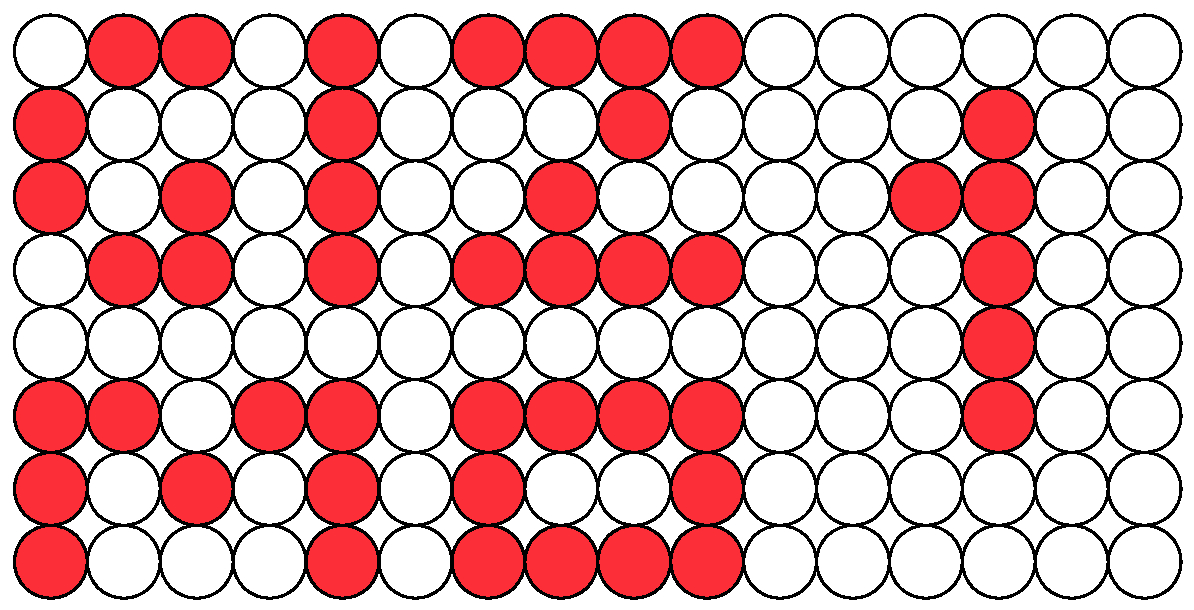
\includegraphics[width=2in]{Gizmo1.pdf}
\vspace{-2em}\caption{\small Boot Screen}\vspace{-2em}
\label{BootScreen}
\end{wrapfigure}

If you power up Gizmo, or press its reset button, it will display its {\bf boot screen}, which includes the version number (at right, the version number is ``1'').

Gizmo will then show the {\bf root menu}.  Use the left potentiometer to scroll to any of the following applications, and use the select button to select an application.  Available applications are:

\subsection{A Bootloader Bug on the Arduino Mega}

Many versions of the Arduino Mega have an error in their bootloader which may cause the Arduino to hang if you've got a MIDI device cables plugged into MIDI IN when you power Gizmo up.  The issue is simple: if on bootup the Mega hears data coming in on MIDI IN (which is its serial port), the bootloader assumes that you're downloading a new program and immediately goes into program-load mode.    But in fact it's probably just MIDI Clock or Active Sensing commands from a chatty synthesizer.  You have four options:

\begin{itemize}
\item Turn on Gizmo without anything plugged into MIDI IN, then plug the cable in.
\item Turn off the synthesizer, turn on Gizmo, then turn the synthesizer back on.
\item Turn on Gizmo with its switch set to ``Prog'', then when it's running, switch it to ``Run''.  I suggest this one.
\item Permanently fix the issue by burning a new bootloader.  This is an involved process, and I don't suggest it.  See https:/\!/github.com/arduino/Arduino/issues/2101
\end{itemize}


%\clearpage

\section{User Interface}

\begin{wrapfigure}{r}{3in}
\vspace{-1.5em}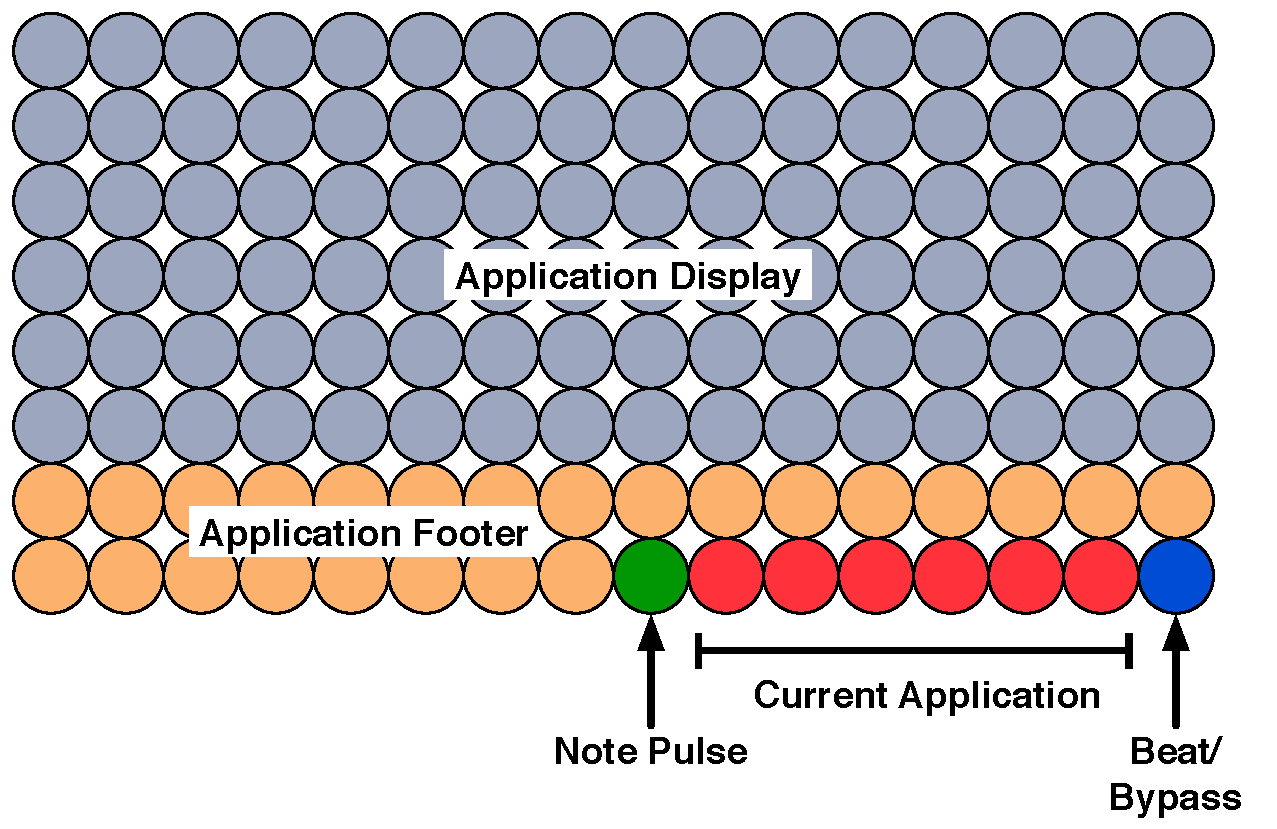
\includegraphics[width=3in]{OverallLayout.pdf}
\vspace{-2em}\caption{\small High-Level Gizmo Layout}
\label{HighLevelGizmoLayout}
\end{wrapfigure}

Gizmo has a modest interface: a 16x8 LED display, two additional on-board LEDs (red and green), three buttons, and two potentiometers (dials): but it strives hard to make good use of these.  

Gizmo's top-level interface layout is a menu hierarchy.  You select menu items, which may take you deeper into the hierarchy, or you can go back up towards the top of the hierarchy.  The top level menu chooses between different {\bf applications}.  Once you have entered an application, its {\bf application number} is displayed in the {\bf current application region} (see Figure~\ref{HighLevelGizmoLayout}).

The current application LEDs light up right-to-left in a certain pattern with increasing application numbers, as shown in Figure~\ref{applicationvalues}.  Gizmo's interface can presently support up to eleven top-level applications.  

\begin{wrapfigure}{r}{1.6in}
\vspace{-3em}\includegraphics[width=1.6in]{Application.pdf}
\vspace{-2em}\caption{\small Application Values}
\vspace{-1em}
\label{applicationvalues}
\end{wrapfigure}

Also shown in Figure~\ref{HighLevelGizmoLayout} are the {\bf Beat/Bypass} light and the {\bf Note Pulse} light.  The Beat/Bypass turns on and off every {\it beat} (quarter note).  This shows the current {\bf tempo}.\footnote{A beat occurs every 24 {\it pulses} of a MIDI Clock or Gizmo's internal clock.}  The Note Pulse light turns on and off every {\it note pulse}: this is the speed you have chosen for the arpeggiator, step sequencer, etc.  Note pulses are defined in terms of note value: for example, if the note pulse is presently in sixteenth notes, then this light will turn on and off four times faster than the beat light, which is in quarter notes. The note pulse light is also affected by the degree of swing (syncopation) you have defined.

If Gizmo's clock is presently {\bf stopped}, either because you have stopped it internally or because Gizmo is being driven by an external MIDI clock which is currently stopped, then {\bf both the Beat/Bypass and the Note Pulse lights will be off} (though if Bypass mode is on, then Beat/Bypass will still blink rapidly).  See Section \ref{startingclock} for more information about starting and stopping the clock.

The reset of the screen is given over to the application.  In many cases an application will display text and other data in the {\bf Application Display} region, and light certain status LEDs in the {\bf Application Footer}.

You wend your way through menus, choose applications, and manipulate them using Gizmo's three buttons and two potentiometers as follows:

\paragraph{Buttons}  The left button is called the {\bf back button}.  The right button is called the {\bf select button}.  The center button is called (unsurprisingly) the {\bf middle button}.   The buttons respond to being {\bf pressed} and immediately released, and also respond to {\bf long presses}: holding a button down for a long time (presently one-half second) and then releasing it. 


Buttons do different things.  Here are certain common items:

\begin{itemize}
\item {\bf Pressing the Back Button}\quad This is the ``escape'' or ``cancel'' button: it {\bf always goes back up the menu hierarchy.}  Thus you can't ever get lost\,---\,just keep pressing the Back button and you'll eventually find yourself at the root menu.
\item {\bf Long-Pressing the Back Button}\quad This toggles {\bf bypass mode}, where Gizmo tries hard to act as if it's just a MIDI THRU coupler between its input and output MIDI wires: it passes through all the MIDI it receives, and with one exception (the Controller, see Section \ref{controller}) it doesn't output any new data.  In bypass mode, the {\bf Beat/Bypass} light (Figure~\ref{HighLevelGizmoLayout}) will stop beating and instead will flash rapidly.
\end{itemize}

\begin{itemize}
\item {\bf Pressing the Select Button}\quad If you're being presented with a menu of options, or a number to choose, or a glyph to choose, the Select button will select the currently-displayed option.  In some applications (such as the Step Sequencer, Arpeggiator, and Recorder) the Select Button is assigned other tasks.
\item {\bf Pressing the Middle Button}\quad Likewise if you're being presented with a menu of options, or a number to choose, or a glyph to choose, the Middle button will increment the current display (but not select it). 
\end{itemize}

\paragraph{Potentiometers}

Gizmo's potentiometers (or {\bf pots}) do a number of tasks, including scrolling through menu options, moving a cursor horizontally or vertically, or choosing a number.  The left pot does primary tasks, and the right pot assists when appropriate.  Note that these are potentiometers, not encoders: if you start turning one, you may experience a big jump initially.  The potentiometers have a limited range (0...1023), and a significant degree of noise, so realistically they can only choose numbers between 0...256 or so.  If asked to select a {\it big} number, the {\bf left pot} will act as a coarse-level selector, and the {\bf right pot} will fine-tune the number.


\paragraph{On-Board LEDs}

There are two LEDs on-board the SparkFun MIDI Shield.  The {\bf red LED} is toggled on and off to reflect incoming MIDI data.  The {\bf green LED} is toggled on and off to reflect outgoing MIDI data.  

\section{How Gizmo Handles MIDI}

Gizmo listens for certain kinds of incoming MIDI data, then hands it to an {\bf application}, which may in turn send MIDI data out.  Applications can send data out any way they wish, but in many cases they restrict themselves to sending data out only to Gizmo's {\bf default MIDI Out Channel.}  Note data (Note on, Note Off) sent out may also be subject to further user-specified transformation in the form of transposition or volume control.  

\vspace{-0.5em}\paragraph{Channel Data} If the incoming data is {\it channel data} (Note on/off, Aftertouch, Pitch Bend, Program Change, Control Change / NRPN / RPN), most applications will listen to it only if it is from the {\bf default MIDI In Channel}, which can be 1--16, or OMNI (all channels), or OFF (no channels).  Some applications may listen to channel data from certain additional channels: for example the MIDI Thru Facility also listens to data on an additional ``Merge channel''.  {\bf Data from all remaining channels is simply passed through to MIDI Out. }  

\vspace{-0.5em}\paragraph{Clock Data} Gizmo can follow clock data or ignore it and generate its own clock.  Furthermore Gizmo can pass incoming clock data through to MIDI Out, or block it.  Gizmo can also emit its own clock data.

\vspace{-0.5em}\paragraph{Other Data} Most other data is simply passed through from MIDI In to MIDI Out.

\vspace{-0.5em}\paragraph{Bypass Mode} When bypass mode is engaged, all data received is simply passed to MIDI Out.  Applications may still listen to 

\vspace{-0.5em}\paragraph{Controlling Gizmo} One incoming channel can be defined as the {\bf default MIDI Control Channel}.  Data on this channel is used only to manipulate Gizmo (via NRPN or CC), for example, changing a parameter.


\clearpage
\section {The Arpeggiator}

\begin{wrapfigure}{r}{3in}
\vspace{-1.5em}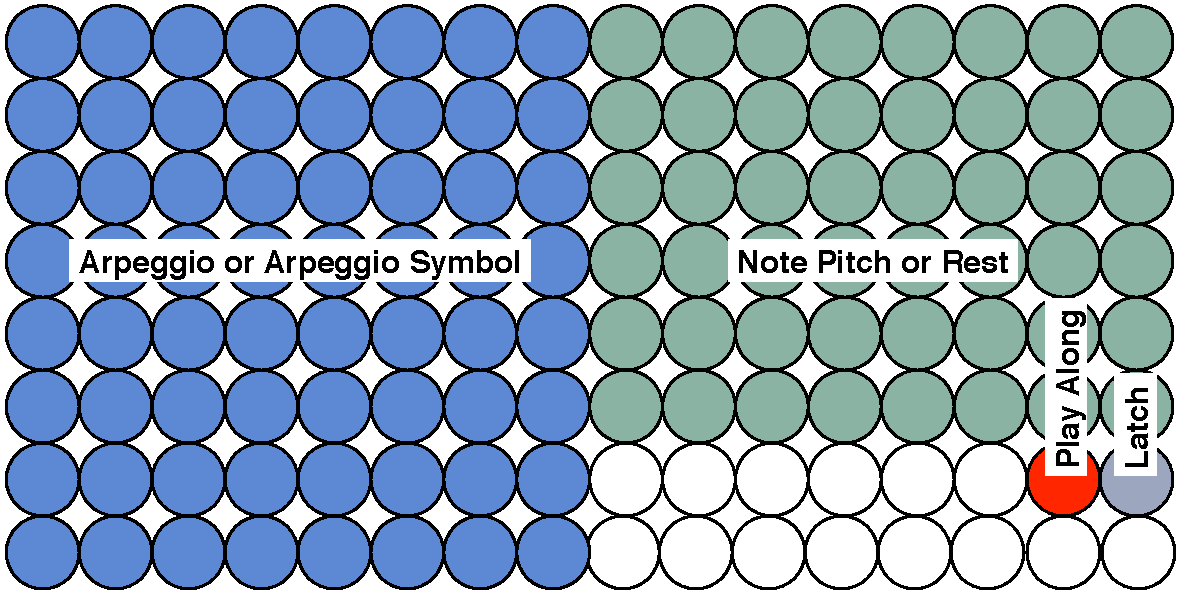
\includegraphics[width=3in]{arpeggio.pdf}
\vspace{-2em}\caption{\small The Arpeggiator Display}\vspace{-1em}
\label{arpeggiator}
\end{wrapfigure}

The arpeggiator allows you to play different kinds of arpeggios, and also to create and save up to ten of them.  The arpeggiator's main menu lets you choose to play five different kinds of pre-set arpeggios, or to select an arpeggio from user-created arpeggio slots 1--10, or finally to create an arpeggio.

An arpeggio is a pattern for repeatedly playing the notes in a chord.  When you hold down a chord on the keyboard, the arpeggiator uses this pattern to play the notes, typically one at a time, according to the pattern selected.  Patterns do not specify exact notes, but rather note orderings.  For example, an arpeggio might be defined as 1, 2, 2, 3, 4, 2, 3: if 1 is set to be the root (lowest) note of your chord, then if you play a C7 chord (C E G B$\flat$), then the arpeggiator will repeat the sequence C E E G B$\flat$ E G.  This pattern will repeat as long as you hold down the keys in the chord.  

Alternatively if you toggle the {\bf latch}, then the playing will continue after you have released the keys, and will only shift to a new chord when you release all notes and then hold down an entirely new chord.  Latch mode is toggled by pressing the Middle button while playing an arpeggio.  When Latch mode is engaged, an LED will light as shown in Figure~\ref{arpeggiator}.

\begin{wrapfigure}{r}{2.7in}
\begin{center}
\vspace{-2em}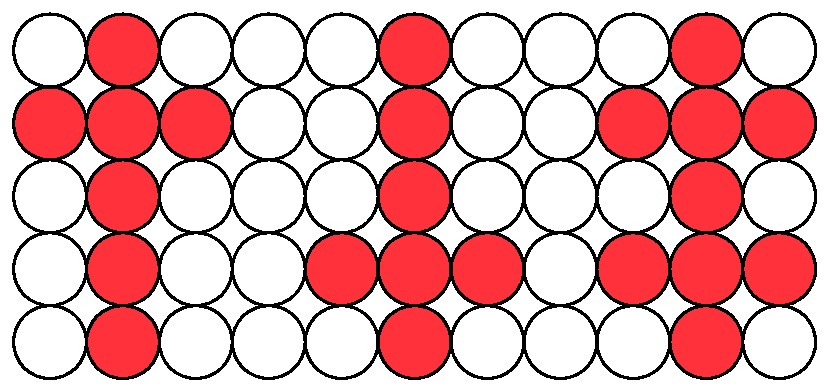
\includegraphics[width=1in]{updown}
\vspace{-1em}
\caption{\small Up, Down, and Up-Down Symbols}
\vspace{-3em}
\end{center}
\end{wrapfigure}


Also, normally you toggle {\bf bypass mode} by Long-Pressing the back button.  But that's not fast enough to turn arpeggiation on and off in performance.  So the arpeggiator also lets you toggle bypass by pressing the {\bf select} button.  (Of course you can also toggle bypass via NRPN if you like). 


\paragraph{Playing Preset Arpeggios}

There are six preset arpeggios: {\it up}, {\it down}, {\it up-down}, {\it random}, {\it chord repeat}, and {\it assign}.  They work as follows:

\begin{itemize}
\item {\bf Up}.  Each note in your chord is played in turn, lowest note first.  When all notes are exhausted, the pattern is repeated.
\item {\bf Down}.  Each note in your chord is played in turn, highest note first.  When all notes are exhausted, the pattern is repeated.
\item {\bf Up-Down}.  Each note in your chord is played in turn, lowest note first, up to but not including the highest note.  When all notes are exhausted, all notes in the chord are played in turn, highest note first, down to but not including the lowest note.  When all notes are again exhausted, this pattern repeats.

\item {\bf Random}.  Chord notes are played at random.  Gizmo tries to not play the same note twice in a row.
\item {\bf Chord Repeat}.  The entire chord is repeatedly played in its entirety.
\item {\bf Assign}. Each note in your chord is played in turn, in the order in which you had pressed the keys when you formed the chord.  When all notes are exhausted, the pattern is repeated.
\end{itemize}

As you play a preset arpeggio, the notes played by the arpeggio will appear at right.  The symbol representing the preset will appear at left.

While playing a preset arpeggio, you can select the number of octaves by choosing calling up the menu by Long-Pressing the Select button, then choosing {\bf Octaves}.  If you have an octaves value \(\geq 0\), then when the arpeggiator exhausts its notes, it will repeat them again one octave higher, then another octave higher, and so on, up to the number of octaves chosen. You an select any value from 0--6 octaves.\footnote{Note that this means that if your chord is larger than one octave, you may not get what you expected.  For example, if you are playing UP with C5 E5 G5 D6, and with octaves\(=\)1, then the arpeggiator will play C5 E5 G5 D6 C6 E6 G6 D7.  Note that C6 is played after D6 is played.  That's the current behavior right now anyway.}

By default the key velocity\footnote{By velocity we mean in the MIDI sense: how fast the key is struck; this basically translates to loudness.} that {\it all} notes in the track will use (as a value 0...127) is determined by the {\bf first note} you press when you hold down a chord.  This strategy usually works well, but if you can instead fix the velocity to a specific value by (once again) calling up the menu by Long-Pressing the Select button, then choosing {\bf Velocity}.  At the far highest end of the velocity options is \texttt{FREE}, which means that the velocity is determined by your fingers again (this is the default).

\paragraph{Creating an Arpeggio}

The last menu option in the top-level Arpeggiator menu is {\bf Create}.  If you choose this, you can create an Arpeggio.  To do this you enter notes one by one.  These won't be the {\it actual} notes that are played when you hold down a chord.  Rather, after you save the result, the Arpeggiator will compact these notes into a sequence of consecutive numbers.  For example, if you play C3 E3 G3 E3 G2, then the Arpeggiator will compact these into 2 3 4 3 1.  Then when you play this as an arpeggio, the Arpeggiator will assign each of these numbers, in order, to the notes in your chord. 

\begin{wrapfigure}{r}{1.6in}
\begin{center}
\vspace{-2em}
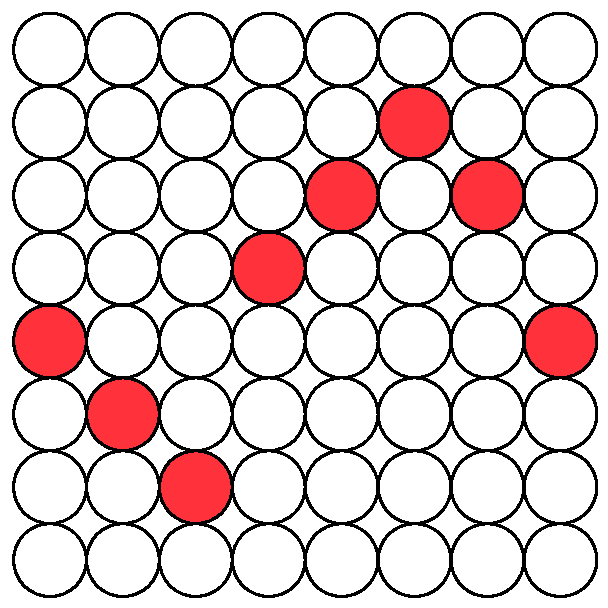
\includegraphics[width=1in]{arpeggioexample.pdf}\\
Example Arpeggio\\[2em]
%\vspace{-1.5em}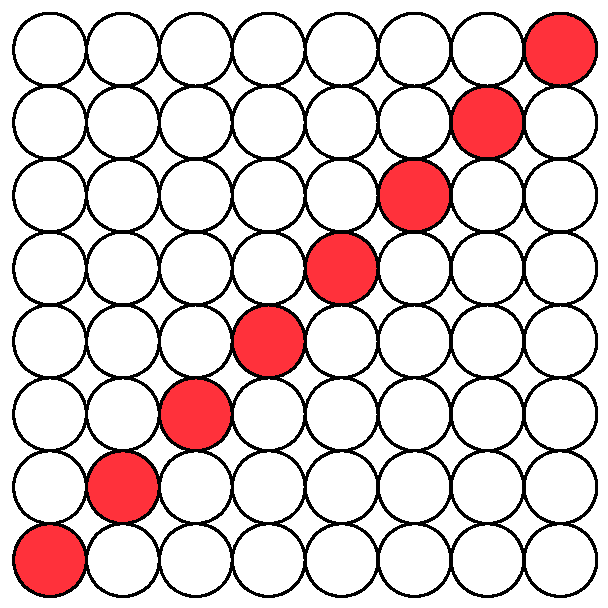
\includegraphics[width=1in]{arpeggioup.pdf}\\
%Ascending Notes\\in Sparse Mode\\[2em]
%\vspace{-1.5em}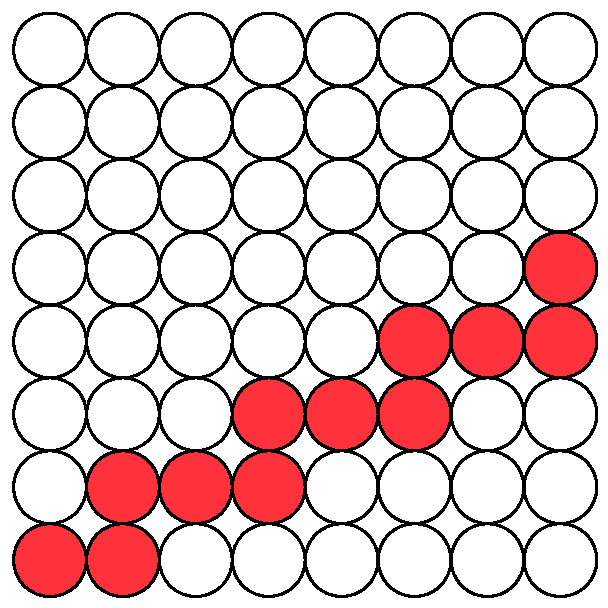
\includegraphics[width=1in]{arpeggiodoubleup.pdf}\\
%Ascending Notes\\in Dense Mode\\
\end{center}
%\vspace{-1em}\caption{\small Example Arpeggio Editing Displays}
\vspace{-2em}
\label{arpeggioediting}
\end{wrapfigure}

The first question you will be asked is \texttt{NOTE}: the Arpeggiator is asking you to specify the note in your arpeggio pattern which will correspond to the root (lowest) note in a played chord.  This allows you to make a pattern which plays notes both above and below the played chord.  For example, if the Root is C3, then the above pattern will instruct the Arpeggiator to play its final note {\it below} the chord root.

After you have entered the root, the Arpeggiator will wait for you to start playing notes.  You can enter a sequence of up to 32 notes, including 15 unique notes (14 on the Mega).  If you enter to many unique notes, or more than 32 notes in total, the Arpeggiator will simply refuse to accept the next note.  You can also enter rests by pressing the Middle button.  On the Mega you can also enter ties (stretching the last note) by long-pressing the Middle button.  The first note may not be a tie: what would it be tying?

\begin{wrapfigure}{r}{3.5in}
\begin{center}
\vspace{-2.5em}
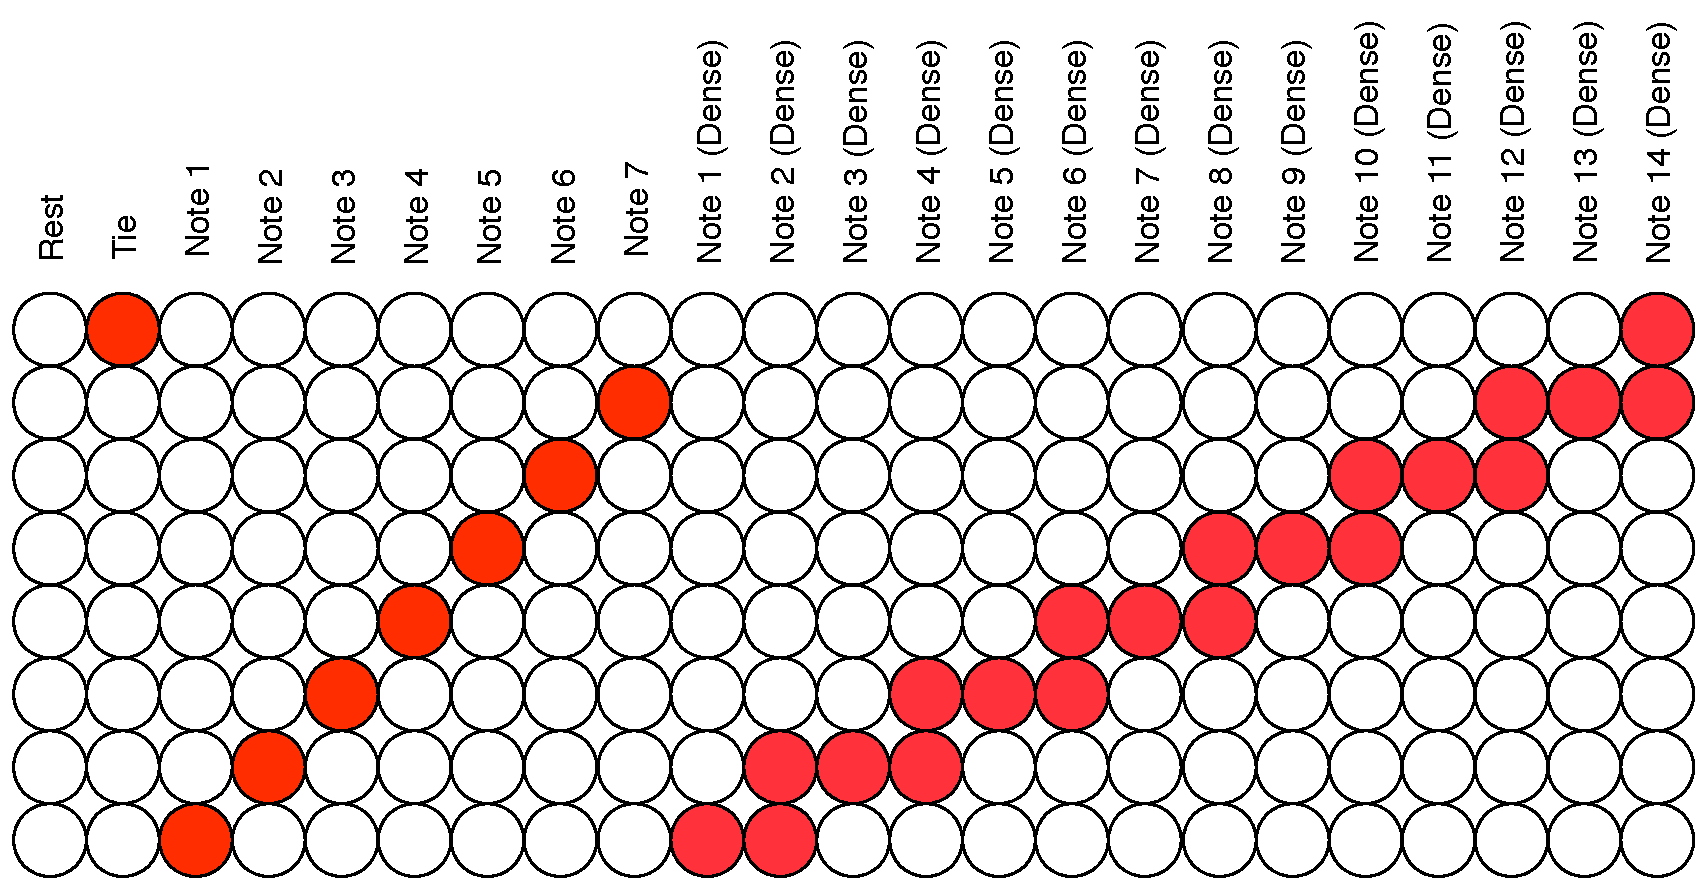
\includegraphics[width=3.5in]{arpeggionotes.pdf}\\
\end{center}
\vspace{-1em}\caption{Displayed arpeggio notes.  If you have entered more than 7 unique notes, the arpeggio will switch to ``dense mode'' to display them.}
\vspace{-1em}
\label{arpeggionotes}
\end{wrapfigure}


As you enter notes, they are displayed in the left half of the LED, and the latest note pitch is displayed in the right half. Figure~\ref{arpeggioediting} shows different arpeggio patterns.  If you have eight or fewer unique notes in your pattern, then they will be displayed in {\it sparse mode} as shown at right.  If you have over eight notes, they will be displayed in {\it dense mode} in order to show all of the notes.  The LEDs don't show the notes per se, but rather the consecutive numbers that the notes represent.  For example, the ascending notes shown at right could be C, D, E, F, G, A, B, C, or they could be C, C\(\sharp\), D, D\(\sharp\), E, F, F\(\sharp\), B.

If you don't like the latest portion of your arpeggio, you can scroll the cursor back to an earlier section by turning the right knob.  Then if you start playing, the later notes will be discarded and the arpeggio pattern will continue from where the cursor was.  You can also scroll to view your past notes, then scroll all the way back to continue.

An {\bf important note regarding the scrolling.}  The cursor is always located at the position where new notes will be entered.  But as you scroll back and forth, you'll hear the notes of your arpeggio.  When you scroll and hear a note, that note is the note {\it immediately before} the cursor position.  It's the last note in the arpeggio before you start adding new notes. It is {\it not} the note that you'll replace when you start entering notes. 

Anyway, when you are satisfied with your arpeggio, Long-Press the Select button to save.  You'll be asked for a slot to save in, and after that, you'll be back in the main Arpeggiator menu.

\paragraph{Playing a User-Created Arpeggio}

To play a user-created arpeggio, from the main Arpeggiator menu, choose one of the numbers 0--9, each of which represents the arpeggiator slot you had saved your arpeggio in (these options appear after the preset options).  Then hold down a chord!  As you play a user-created arpeggio, the notes played by the arpeggio will appear at right.  The arpeggio pattern will scroll by at left.


The preset arpeggio patterns (such as Up-Down) vary with the number of notes in your chord: if you hold down five notes for example, and octaves=0, then five notes will be played in the arpeggio pattern.  This isn't the case for user-created arpeggios, which have a fixed user-specified number of notes.

What happens if your arpeggio is designed for three notes but you hold down  five notes in your chord?  Only three of your five notes will be played.

What happens if your arpeggio is designed for five notes but you hold down only three notes in your chord?  Then notes from the bottom (or top, as appropriate) of your chord will be transposed up/down one octave to make up the remaining notes.

Also, because they are fixed in size, user-created arpeggios do not respond to the octaves option.

\paragraph{More Arpeggiator Options}

In addition to Octaves, the arpeggiator menu (Long-Press the select button) also includes the Options Menu as a submenu.\footnote{Recall that the Options Menu is for options shared among several applications: that's why it's a separate menu.  That and code space issues.}  See Section \ref{options} for detailed information on each of the options.  The Arpeggiator responds to the following options:

\vspace{0.75em}
\begin{tabular}{lllll}
Tempo& Note Speed& Swing & Note Length&Transpose (on Mega)\\
In MIDI& Out MIDI&Control MIDI&MIDI Clock&Volume (on Mega)\\
\end{tabular}

\vspace{0.75em}
Of particular interest to you may be Length and Tempo.  And Swing!

One note regarding the {\bf Note Length} option.  If the Note Length is set to 100 (and {\it only} 100), the Arpeggiator behaves specially: each note will extend until the next note (or rest) is played, regardless of how long that is.  Thus if you have Swing turned on, notes will extend until the next syncopated (delayed) note even if their time is up. This provides a fully legato feel.


\paragraph{The Left and Right Knobs}  When playing an arpeggio, turning the left knob will transport you directly to the Tempo menu option, so you can easily change the note tempo.  Similarly, turning the right knob will send you to the Note Length menu option.  You'll have to turn a lot to get this to happen (as a safety precaution).\footnote{{\it What about Arpeggio Key Velocity?  Swing?  Note Speed? Velocity or Transpose?}\qquad Arpeggio Key Velocity's easy: just press the select button twice.  For the others you'll have to go through the options menu, sorry.  Though it's easy to modify Gizmo to change this.}  Once you're done changing the tempo or note length, press the Select button to save it, or the Back button to cancel and return to your previous value.

\clearpage


\begin{wrapfigure}{r}{3in}
\vspace{-1.5em}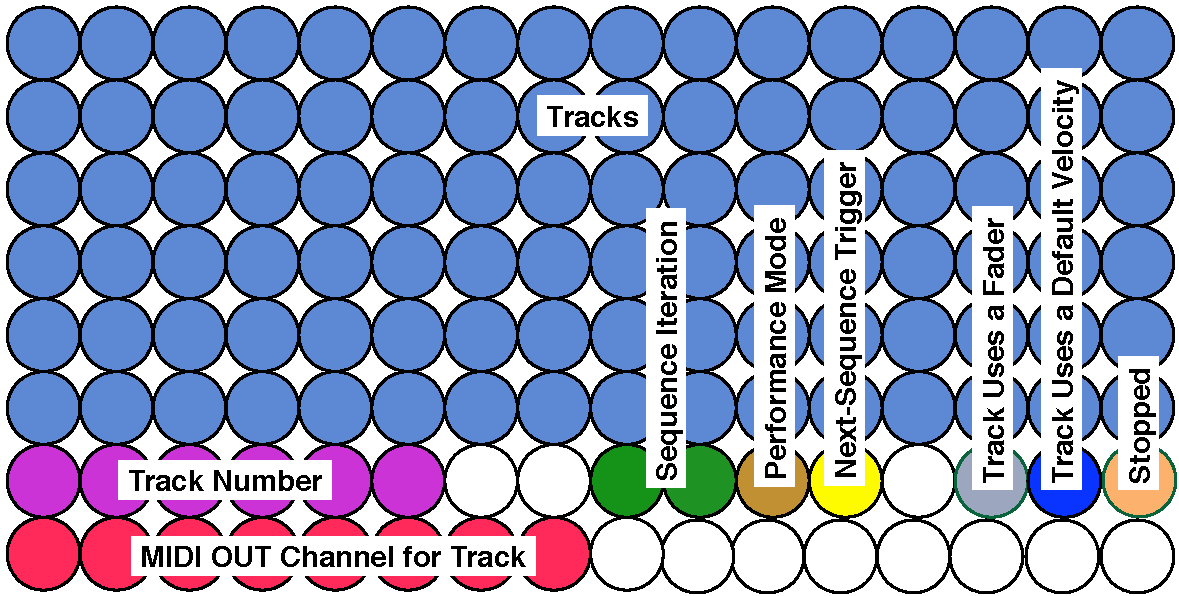
\includegraphics[width=3in]{stepsequencer}
\vspace{-2em}\caption{\small Step Sequencer Display}\vspace{-1em}
\label{stepsequencer}
\end{wrapfigure}



\section {The Step Sequencer}

The Step Sequencer makes it easy to create multitrack loops common on devices like drum machines.  On the Uno, you can have twelve 16-note tracks, eight 24-note tracks, or six 32-note tracks.  On the Mega you can additionally have four 48-note tracks or three 64-note tracks.

\begin{wrapfigure}{r}{1in}
\vspace{-1em}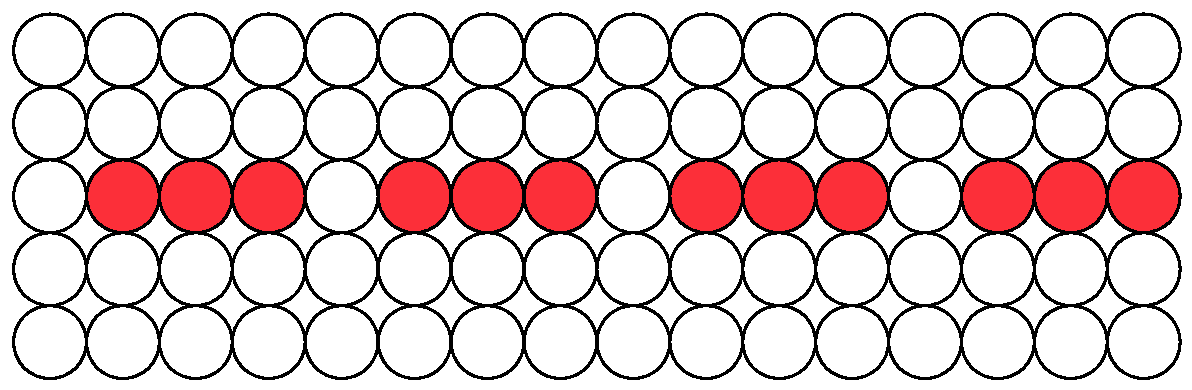
\includegraphics[width=1in]{none.pdf}
\vspace{-2em}\caption{\small None}\vspace{-1em}
\label{none}
\end{wrapfigure}

When you choose the Step Sequencer from the root menu, you will be asked to load a sequence from a slot.  You can do this, or you can create a new empty sequence by choosing \texttt{-~-~-~-} (meaning {\it none}).  Slots are displayed by number, plus an \texttt{L} (for Load) and an optional \texttt{R} (for Recorder) or \texttt{S} (for Step Sequencer) if the slot already has a file from one of the two applications.  This letter {\bf blinks} if the file isn't the type of your current application to warn you that you might eventually overwrite a slot when you save.

If you have chosen {\it none}, or have chosen an empty slot or one presently filled by the Recorder, you'll be asked to initialize the sequence first, choosing from 16, 24, 32, or (on the Mega) 48 or 64 notes per track. Then you are taken to the main Step Sequencer display.  

Figure~\ref{stepsequencer} shows the general step sequencer display structure.  The {\it Tracks} region is where sequencer tracks are displayed and edited.  The {\it Track Number} area tells you the number of the currently-edited track.  Figure~\ref{tracknumber} explains how to interpret this.  The {\it Stopped} LED tells you if the step sequencer is currently stopped (or playing).  The {\it Track Uses a Default Velocity} LED tell you if all notes in the current track are fixed to the same velocity, or permitted to use different velocities.  The {\it Track Uses a Fader} LED is lit when the pre-track fader (volume) is set to something other than maximum volume for the current track.  The {\it Locked} LED is lit when you've locked the sequence (new played notes or rests are ignored).  Finally, the {\it MIDI Out Channel for Track} tells you what channel the current track is playing.  The patterns for the MIDI Out Channel for Track are the same as those in Figure~\ref{midichannelvalues}, except that MIDI Out does not support ALL (OMNI).


\begin{wrapfigure}{r}{1.8in}
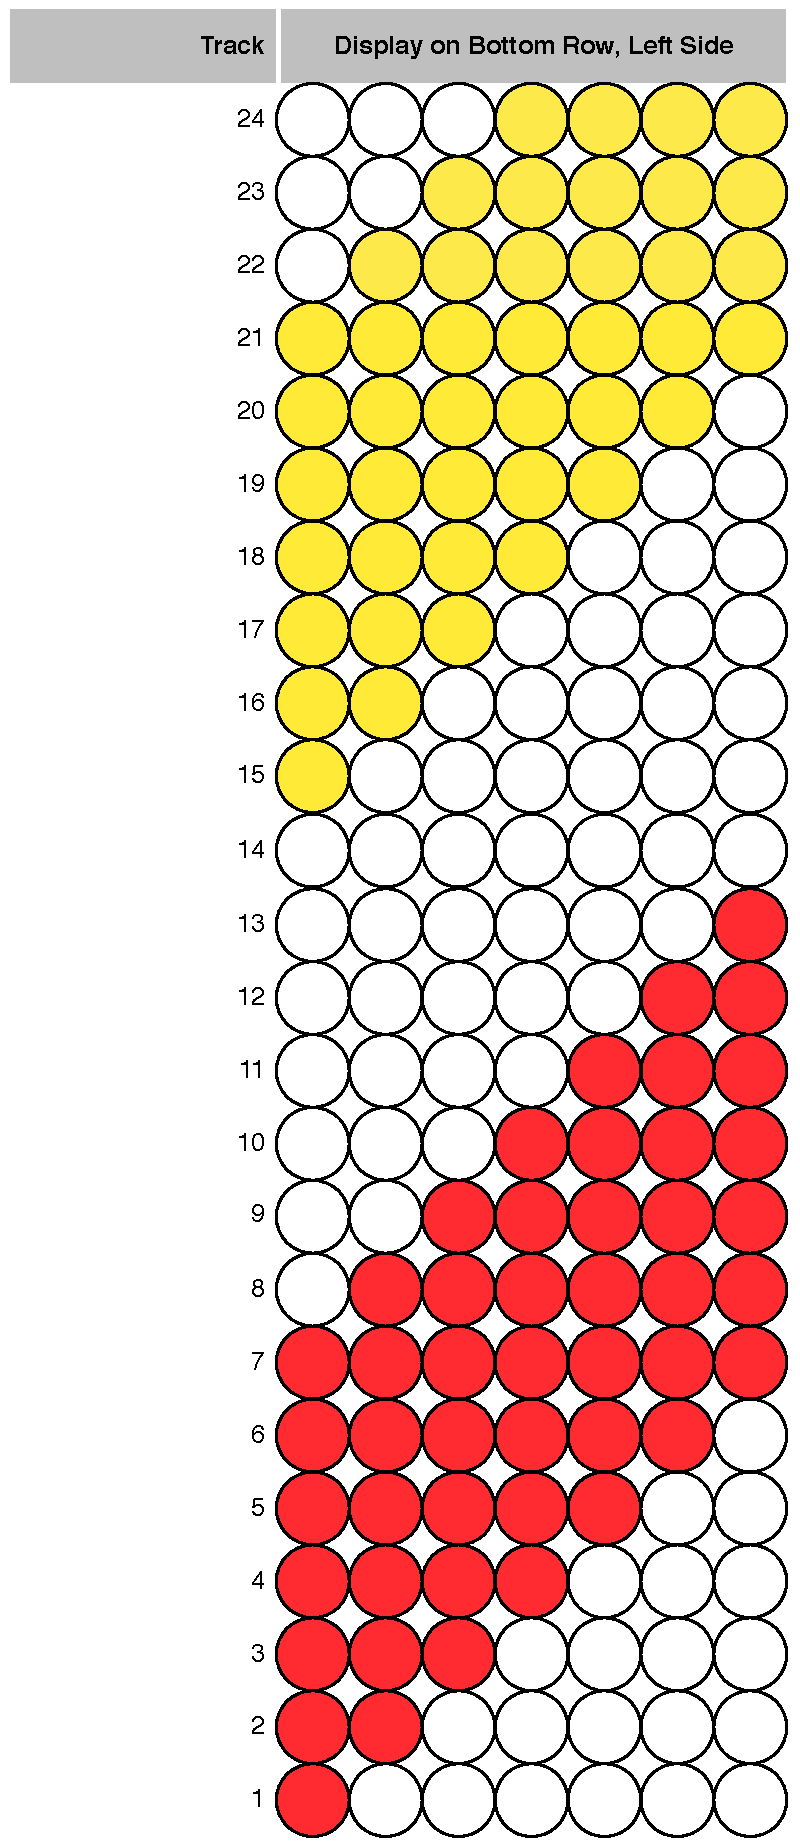
\includegraphics[width=1.8in]{track.pdf}
\vspace{-2em}\caption{\small Track Numbers}
\label{tracknumber}
\end{wrapfigure}

Each track has a blinking {\it edit cursor} which determines, normally, where notes are entered if you play them.  The location of this cursor is determined by the potentiometers.  You select your current track by turning the left knob.  In a given track, you choose the current note position by turning the right knob.  The Tracks region also displays a blinking vertical set of LEDs which indicate which notes in the tracks the Step Sequencer is currently playing.  As the Step Sequencer plays notes, this vertical group heads to the right, eventually wrapping around.  This is the {\it play position cursor}.

Each track takes up one or two rows in the Tracks area: 16-note tracks take a single row, 24-note and 32-note tracks take two rows, 48-note tracks take three rows, and 64-note tracks take four rows.    There might be up to twelve tracks, yet the tracks display region is only six LEDs high.  This of course means that  the Tracks region scrolls as you turn the left knob.\footnote{This also means that can only see one 64-note track at a time.  BTW, you might be interested in knowing why Gizmo can't presently do 8- or 12-note tracks.  This is because the memory usage is pretty high\,---\,we're storing a lot of per-track information, and with 8-note tracks you can have 24 of them!  I figure these are not big losses: you can always do 16 or 24 notes instead.  

There's a different reason we don't have 128-note tracks: one track would take up the entire screen, including any footer information.  Also, you'd only have a single track, which seems to me to be not particularly useful.}

You enter notes by moving the edit cursor to the a location, then pressing keys.  You can also press the Middle Button to enter a rest, or Long Press the Middle Button to enter a {\it tie}.  A tie just means ``keep playing the previous note'': it essentially lengthens the previous note.  You can enter multiple ties in series to make a note as long as you like.

\enlargethispage{1em}

Pressing the Select button will toggle whether the Step Sequencer is playing.  When you start playing the Step Sequencer, it waits for the clock to reach a measure boundary before beginning.  Furthermore, even if you start playing the Step Sequencer, if the clock isn't running it won't play at all.

\paragraph{Play Position Mode}

If you turn the right knob fully to the left, you will find that the cursor scrolls right off the left side of the screen.  At this point you are in {\bf play position mode}.  Here, if you press a key, it is entered at the play position cursor.

\begin{wrapfigure}{r}{1.25in}
\vspace{-1em}\hspace{\fill}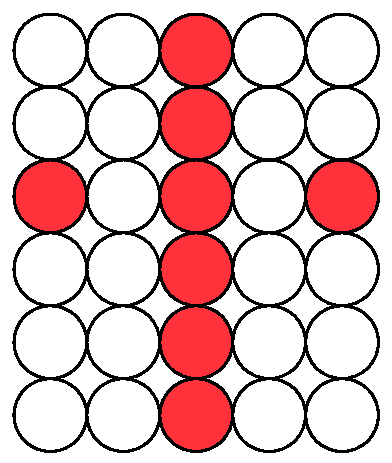
\includegraphics[width=0.7in]{playpositionmode}\hspace{\fill}%
\vspace{-1em}
\caption{\small The Play Position Mode Cursor.  The current track is marked by the two dots.}\vspace{-1em}
\label{playpositionmode}
\end{wrapfigure}


In play position mode, the function of the Middle Button changes.  Now if you press the Middle Button, it will toggle muting the current track.  You can tell a track is muted because the LEDs at each end of the track are blinking.  Additionally, if you Long Press the Middle Button, it will erase all the notes on the current track (but not change its settings).

You can tell you're in play position mode because the play position cursor has changed to include two dots which indicate the current track, as shown in Figure~\ref{playpositionmode}.

Play position mode isn't all that easy to enter notes, particularly if there is any degree of swing: I'd stick with the normal mode.  You can get out of play position mode just by turning the right knob so that the edit cursor is once again on-screen.

\paragraph{Other Types of Track Data}  A track can store and sequence other kinds of data besides Note-On and Note-Off.  Specifically, you can set a given track to store and replay any one of (raw) CC, 14 Bit CC, NRPN, RPN, Pitch Bend, Channel Aftertouch, or Program Change commands by choosing {\bf Type} from the menu (see {\bf Menu Options} below).  If you select (raw) CC, 14 Bit CC, NRPN, or RPN, you will be further prompted to specify which parameter number you'd like to sequence (for example, CC\# 42 or NRPN\# 12312).

Non-note data is entered differently than note data.  To enter non-note events, send an event to the MIDI In Channel, then press the {\bf middle button}: the most recent sent event will then be recorded at the current position.  You can erase data at the current position (essentially send a rest) by long-pressing the middle button.\footnote{This may be confusing as rests are entered by simply {\it pressing} the middle button for note data, but I figured entering data was more important than entering rests in the non-note case.  Sorry.}

Some notes.  First, if you sent a Polyphonic Aftertouch event (on any key) it will be recorded instead as Channel Aftertouch.  Second, if your track is configured for (raw) CC, then you can send {\it any} raw CC value to it (all 127 parameter numbers), and it will also emit the same; but if your track is configured for 14-bit CC, then only the first 31 parameter numbers may be used.  Third, any Pitch Bend value can be stored except for 8191 (the high value).  Fourth, any 14 Bit CC, RPN, or NRPN value can be stored except for 16383 (again, the high value).  

\paragraph{Menu Options}

If you Long Press the Select button, you'll call up the Step Sequencer's menu.  The Step Sequencer has a number of options:

\begin{itemize}
\item {\bf Solo} (or {\bf No Solo})\quad This plays only the current track, muting the others.
\item {\bf Length}\quad This specifies the note length of notes in the track, as a percentage (0 is fully staccato and 100 is fully legato).   You can choose numerical values, or choose \texttt{DFLT}, which tells the Step Sequencer to use the default note length specified in the Options menu (see Section \ref{options}).
\item {\bf Out MIDI (Track)}\quad This specifies the MIDI Out Channel for notes in the track,    You can choose a value 1...16, or choose \texttt{DFLT}, which tells the Step Sequencer to use the default MIDI Out Channel specified in the Options menu (see Section \ref{options}).
\item {\bf Velocity}\quad This lets you specify a key velocity\footnote{By velocity we mean in the MIDI sense: how fast the key is struck; this basically translates to loudness.} that {\it all} notes in the track will use (as a value 0...127).  If you would instead prefer that each note in the track use its own independent key velocity as you had entered them, you can choose \texttt{FREE}.
\item {\bf Fader}\quad This lets you specify a volume modifier which is multiplied against the velocities of the notes in the track.  Possible values are 0...127, where 0 completely hushes the notes, and 127 lets them play at their specified velocities. 
\item {\bf Reset Track}\quad This wipes out and resets the track.  Unlike Long-Pressing the Middle Button while in Play Position mode, this doesn't just clear the track: it also resets all of its settings to their defaults.
\item {\bf Save} \quad This saves the sequence. You then choose the slot to save in.  Slots are displayed by number, plus an \texttt{S} (for Save), plus optionally an \texttt{R} or \texttt{S} (for Recorder or Step Sequencer) if the slot is already used by that application.  This letter {\bf blinks} if the file isn't the type of your current application to warn you that you will be overwriting the other application's slot.
\item {\bf Type} (Mega only) \quad Lets you specify the type of data stored in this track.  See {\bf Other Types of Track Data} above.
\item {\bf Clock Control} (or {\bf No Clock Control}) (Mega only) \quad This toggles {\it clock control mode}.  Normally, if you play or stop the sequencer, it will not send MIDI STOP or MIDI PLAY commands\,---\,if you want to start the MIDI clock you have to do so separately (see Section \ref{startingclock}).  However it's common for sequencers to issue these commands when you start or stop the sequencer, so as to also start or stop other sequencers listening over MIDI.  To do this, turn on clock control mode.  Note that this only has an effect if Gizmo is {\bf generating} a MIDI Clock (see ``MIDI Clock'' in Section \ref{options}).  Finally note regardless of the setting of this options, if Gizmo is {\it using} an external MIDI Clock (again, see ``MIDI Clock'' in Section \ref{options}), the Step Sequencer will stop and start in response to incoming MIDI Clock commands.
\item {\bf Lock} (or {\bf Unlock}) (Mega only) \quad This toggles {\it locked mode}.  Here, playing a note will not enter it into the sequence, nor will you be able to enter a rest or clear the track.  You will be able to reset the track and perform any other operation.  Note that track locks must be saved with your sequence: if you lock (or unlock) a sequence, but don't save, then next time the sequence will be back in its previous unlocked (or locked) state.

While in locked state, you can {\bf transpose} the sequence by playing a key.  The sequence is transpose by the difference between your key and middle C.  Reset the transpose by pressing middle C.  This transposition is on top of the global transposition in the Options menu.

\item {\bf No Echo} (or {\bf Echo}) (Mega only) \quad This toggles {\it no-echo mode}.  Normally when you enter a note, it's automatically played so you get some feedback.  But in some circumstances this isn't desirable: for example, if you're entering {\it and} playing notes from the same keyboard, then this default behavior will cause two notes to be played whenever you enter a note.  {\bf No Echo} will turn this off.\footnote{The Mega also has another closely related feature: if you're in play position mode and you have entered a note slightly before its time, Gizmo won't play it (the first time) when its time comes up, because you just played it yourself.  This isn't the case on the Uno: you'll hear a double-played note the first time.  There's not enough space on the Uno to add this feature, sorry.}
\item {\bf Options} \quad This brings up the Options menu, which enables you to do...
\end{itemize}

\paragraph{More Step Sequencer Options}

Beyond the settings above, the step sequencer responds to a number of options in the Options Menu.  See Section \ref{options} for detailed information on each of the options.  The Step Sequencer responds to the following options:


\vspace{1em}
\begin{tabular}{llllll}
Tempo& Note Speed& Swing & Note Length&Transpose (on Mega)&Click\\
In MIDI& Out MIDI&Control MIDI&MIDI Clock&Volume (on Mega)\\
\end{tabular}

\vspace{1em}
Of particular use are Tempo, Note Speed, Swing, and especially Click.


\clearpage

\section {The Note Recorder}

\begin{wrapfigure}{r}{3in}
\vspace{-1.5em}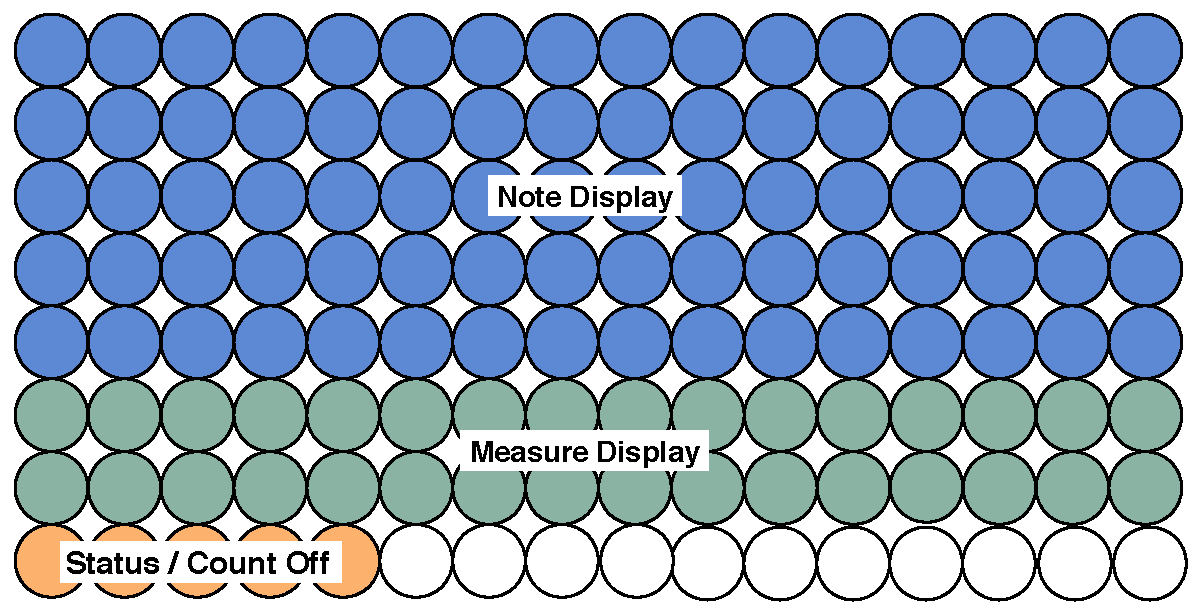
\includegraphics[width=3in]{recorder.pdf}
\vspace{-2em}\caption{\small Recorder Display}\vspace{-1em}
\label{recorder}
\end{wrapfigure}

The Note Recorder lets you record and play back approximately 64 notes\footnote{Why {\it approximately} 64? Because the recorder is recording MIDI NOTE ON and NOTE OFF messages.  If you provide 64 pairs of these messages, it'll take up exactly all the available memory.  But you could plausibly send a few more NOTE ON than NOTE OFF messages, in which case at the end of the recording all the remaining outstanding notes will be terminated.  This would allow you to squeeze in a few (perhaps 16) more notes in rare circumstances.  But I'd not rely on it.  BTW, if you looked carefully you would have noted that the Note Display in Figure~\ref{recorder} has space for 16 more notes too.} spread over 21 measures.\footnote{Why 21?  Because notes are stored with a timestamp of eleven bits, resulting in \(2^11 = 2048\) timesteps.  A single timestep is 1/24 of a quarter note, and a quarter note is 1/4 of a measure, so we have \(2048 / 24 / 4 = 21 1/3\) measures.  We round that down to 21.}  You can save up to two recordings on an Arduino Uno and nine recordings on a Mega.

The Note Recorder screen has two major parts.  The {\it Note Display} section indicates the current note number being played (and hints at the remaining notes available).  The {\it Measure Display} section indicates the current measure being played (and again hints at the remaining measures available).  When recording a song, each of these sections will contain a single lit LED indicating the current note or measure position.  When playing a song, the Note Display and Measure Display will each also contain an additional lit LED indicating the position of the end of the song.

\begin{wrapfigure}{r}{1in}
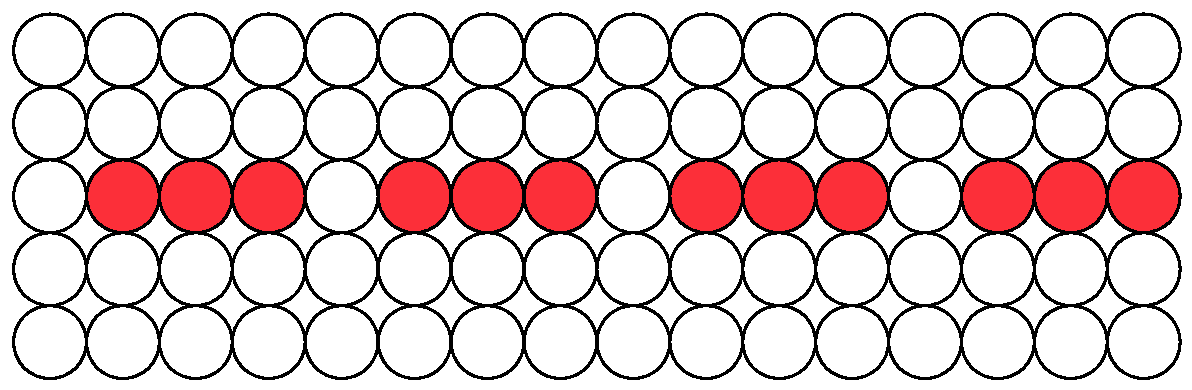
\includegraphics[width=1in]{none.pdf}
\vspace{-2em}\caption{\small None}\vspace{-1em}
\label{none}
\end{wrapfigure}

When you choose the Note Recorder from the root menu, you will be asked to load a recording from a slot.  You can do this, or you can create a new empty recording by choosing \texttt{-~-~-~-} (meaning {\it none}).  Slots are displayed by number, plus an \texttt{L} (for Load) and an optional \texttt{R} (for Recorder) or \texttt{S} (for Step Sequencer) if the slot already has a file from one of the two applications.  This letter {\bf blinks} if the file isn't the type of your current application to warn you that you might eventually overwrite a slot when you save.

\begin{wrapfigure}{r}{1.5in}
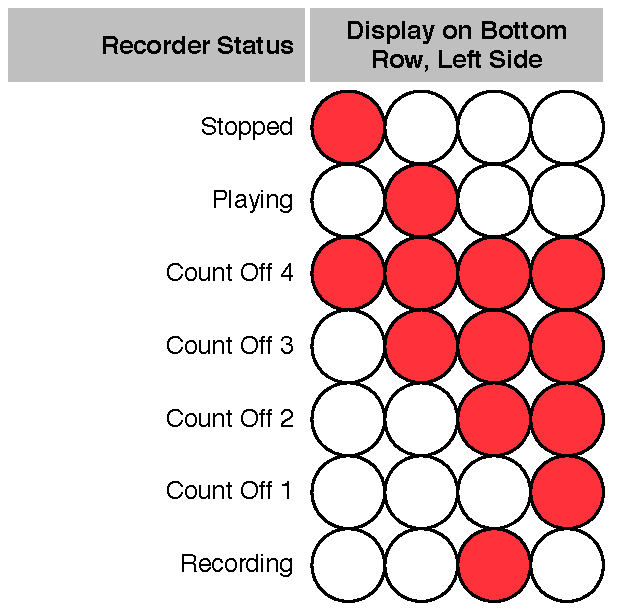
\includegraphics[width=1.5in]{recorderstatus.pdf}
\vspace{-2em}\caption{\small Recorder Status LEDs}\vspace{-4em}
\label{recorderstatus}
\end{wrapfigure}

After this you will enter the Note Recorder.  The Note Recorder is always in one of four states, indicated the patterns at right:

\begin{itemize}
\item Stopped
\item Playing
\item Counting off beats prior to Recording
\item Recording
\end{itemize}

When you enter the Note Recorder, the state is initially Stopped.  To start playing a song, press the middle button.  To stop playing (or stop recording), you also press the middle button.  To start recording a song, Long Press the middle button.  The recorder will count off four beats for you, then start recording.

You can choose {\bf Repeat Mode} from a menu by Long-Pressing the Select (right) Button.  When in repeat mode, the recorder repeats the song it is playing at the measure boundary after it has finished playing the song.  Repeat mode also toggles an LED (see Figure~\ref{recorder}).

You can save your recorded song by pressing the Select Button.  Gizmo will ask you to select a slot to save in, then it will exit the Recorder.  Slots are displayed by number, plus an \texttt{S} (for Save), plus optionally an \texttt{R} or \texttt{S} (for Recorder or Step Sequencer) if the slot is already used by that application.  This letter {\bf blinks} if the file isn't the type of your current application to warn you that you will be overwriting the other application's slot.

\paragraph{More Recorder Options}  
You can also choose the Options Menu from inside the Note Recorder: it's part of the menu brought up by Long-Pressing the Select button.  The Recorder responds to a number of options:

\vspace{1em}
\begin{tabular}{llll}
Tempo&Transpose (on Mega)&Volume (on Mega)&Click\\
In MIDI& Out MIDI&Control MIDI&MIDI Clock\\
\end{tabular}

\vspace{1em}
Of particular use to you will be Tempo and Click.  Click gives you an audible click track: and the count-in is also clicked for you.

\paragraph{Recording and Quantization}

The Recorder records nothing but MIDI NOTE ON and NOTE OFF messages.  It presently quantizes these messages, rounding them up or down to the nearest MIDI Clock pulse, that is, 1/24 of a quarter note.\footnote{This is pretty low-resolution, but there you have it.  Space is tight.}

\vspace{2em}
\begin{figure}[h!]
\begin{center}
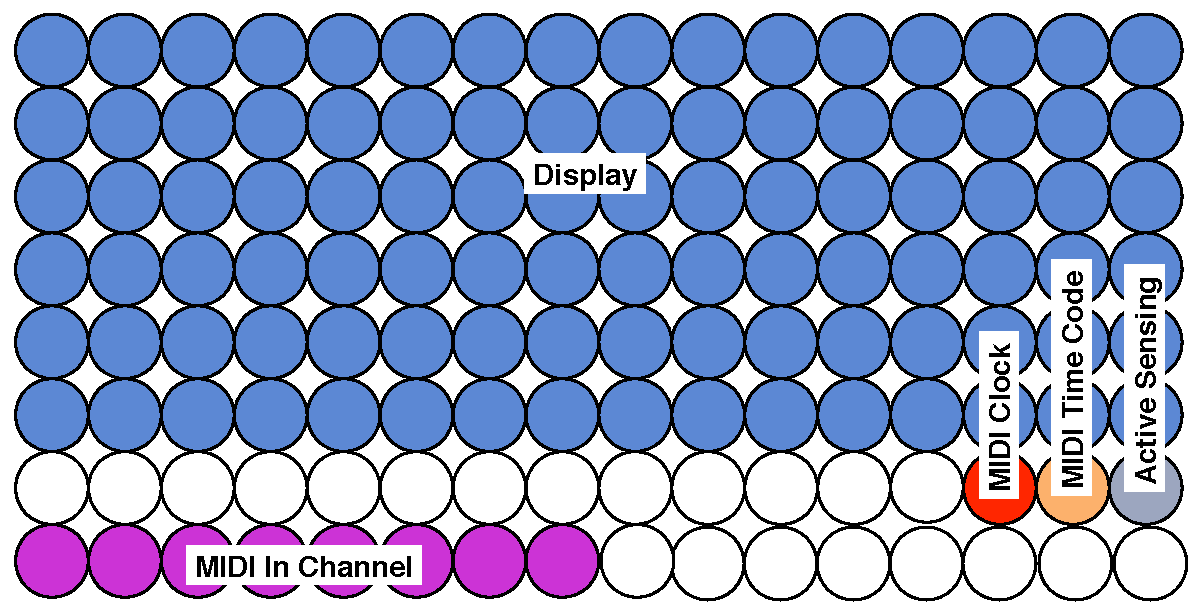
\includegraphics[width=3in]{GeneralGauge.pdf}~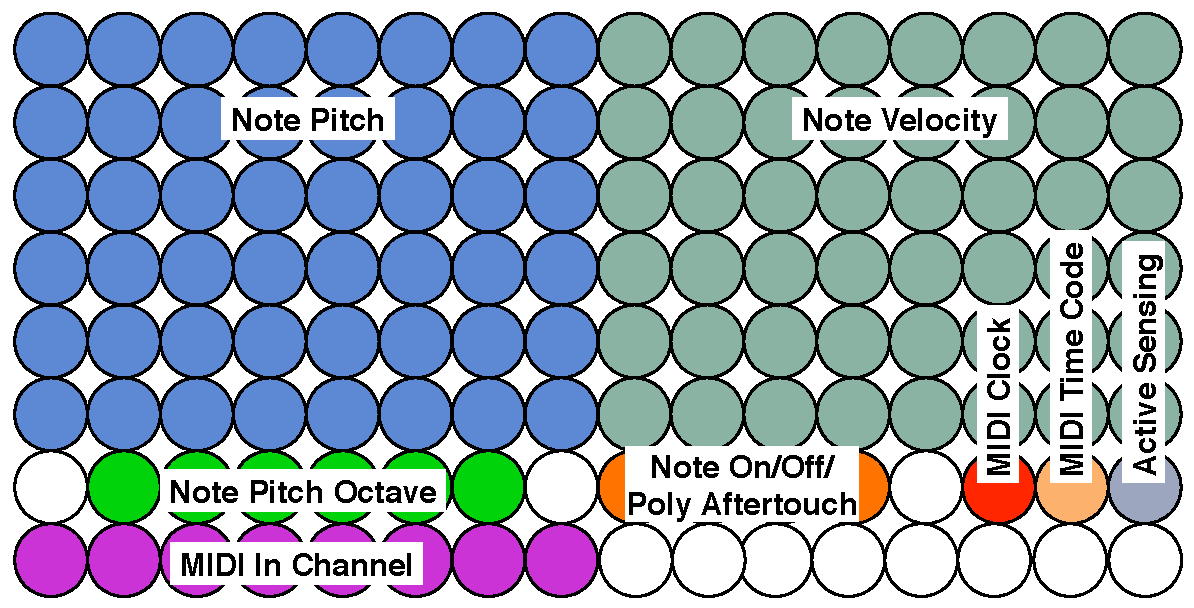
\includegraphics[width=3in]{NoteGauge.pdf}
\caption{\small (Left) General Gauge Display, and (Right) Note Gauge Display}
\label{gaugedisplays} \end{center}
\vspace{-3em}\end{figure}


\section {The MIDI Gauge}


\begin{wrapfigure}{r}{2in}
\vspace{-1.5em}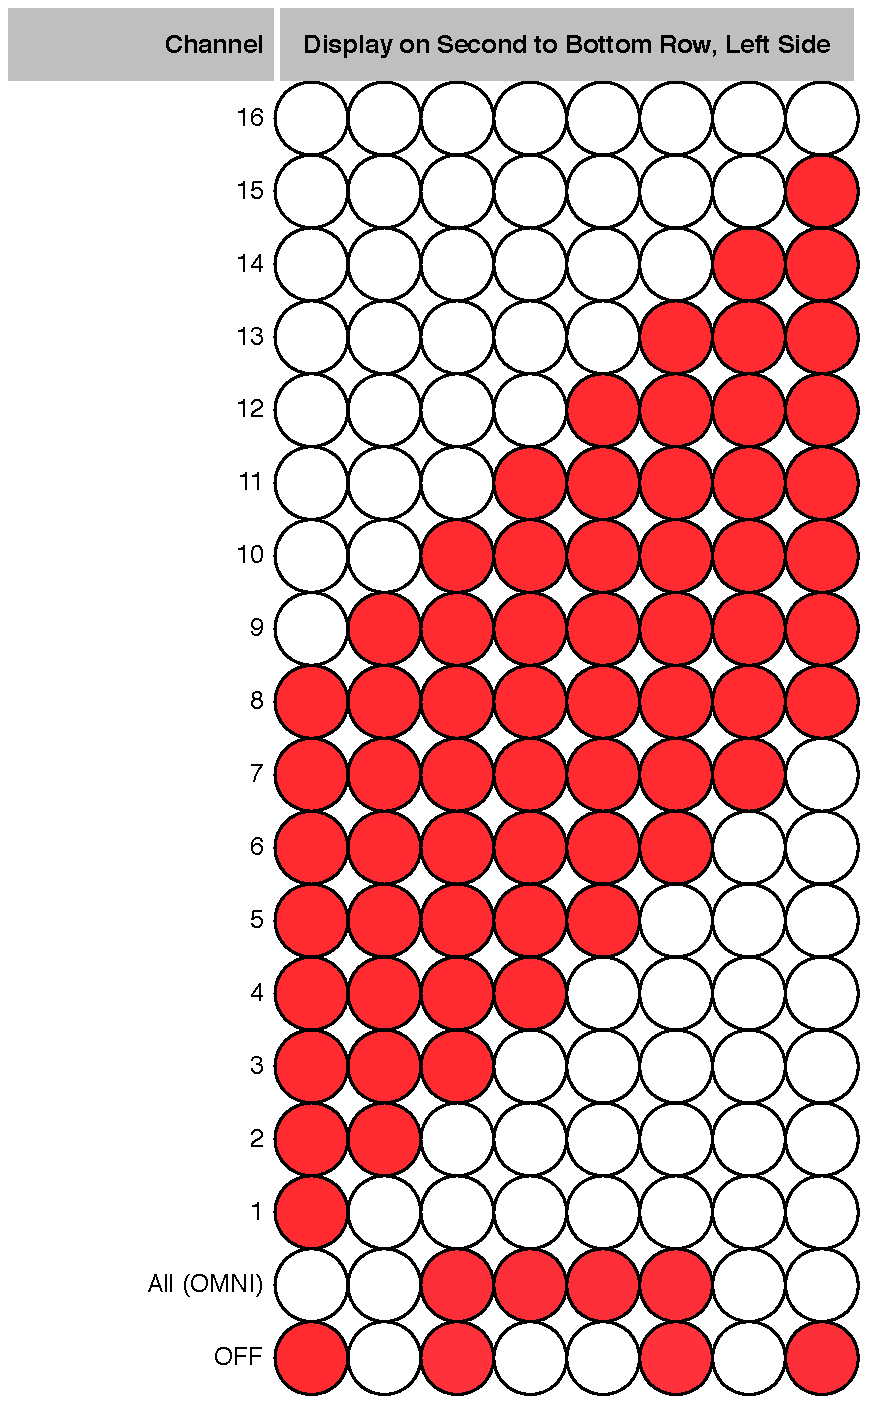
\includegraphics[width=2in]{midichannel.pdf}
\vspace{-2em}\caption{\small MIDI Channel Values}
\label{midichannelvalues}
\end{wrapfigure}


The MIDI gauge listens to incoming MIDI messages and displays them on-screen.  This only occurs if the MIDI IN channel is something other than NO CHANNEL (See {\bf Options\(\boldsymbol\rightarrow\) In MIDI}, in Section \ref{options}).



There are three kinds of MIDI messages for purposes of display.  {\it General} messages take up the whole screen with a single message.  {\it Note} messages split the screen between pitch and velocity of the given note (on, off, polyphonic aftertouch).  Finally {\it Frequent} messages are simply displayed by lighting a specific LED to indicate their presence. 


Messages that are associated with a MIDI channel will have their channel number displayed at bottom left (see Figure~\ref{gaugedisplays}~[Left]).  Note that if the MIDI IN channel is something other than OMNI (ALL Channels), then only messages associated with the MIDI IN channel will be displayed.






\paragraph{General Gauge Display}  These are simple displays which take up the entire screen.

\begin{itemize}
\item {\bf Pitch Bend}\quad The 14-bit value is displayed
\item {\bf Channel Aftertouch}.  \texttt{AT} is displayed, followed by the value.
\item {\bf Program Change}\quad \texttt{PC} is displayed, followed by the value.
\item {\bf Control Change (CC)}\quad If the CC parameter is for 7-bit values, then the value is shown first, then text is scrolled with the value, then \texttt{CC}, then the parameter.  If the CC parameter is for 14-bit values, the MSB of the value is shown first, then text is scrolled with the value, then \texttt{CC}, then the parameter, then in parentheses the 14-bit (MSB+LSB) value.
\item {\bf Registered Parameter Number (RPN)}\quad The value (7-bit MSB only) is shown first, then text is scrolled with the value (MSB), then \texttt{RPN}, then the parameter (14-bit), then in parentheses the 14-bit (MSB+LSB) value.
\item {\bf Non-Registered Parameter Number (NRPN)}\quad The value (7-bit MSB only) is shown first, then text is scrolled with the value (MSB), then \texttt{NRPN}, then the parameter (14-bit), then in parentheses the 14-bit (MSB+LSB) value.
\item {\bf Channel Mode}\quad On the Uno, the channel mode value is shown first, then the text \texttt{CHANNEL MODE}, then the channel mode parameter (120--127).  The Mega is more specific: the meaning channel mode parameter and value are instead shown as a text message (such as \texttt{RESET ALL CONTROLLERS}).  In the case of \texttt{MONO ON} the channel count is shown first.  The Channel Mode parameters are:
\begin{center}\begin{tabular}{@{}rlll@{}}
{\it Parameter}&{\it Value}&{\it Meaning (Displayed On Mega)}\\[0.1em]
\hline\\[-0.9em]
120&Normally 0&All Sound Off\\
121&Normally 0&Reset All Controllers\\
122&0=Off, 1=On&Local Control Off ({\it or} On)\\
123&Normally 0&All Notes Off\\
124&Normally 0&Omni Off\\
125&Normally 0&Omni On\\
126&\(C\)&Mono On ({\it with \(C\) channels, shown first})\\
127&Normally 0&Poly On\\
\end{tabular}\end{center}
\item {\bf System Exclusive}\quad \texttt{SYSX} is displayed.\footnote{Note that the version of the MIDI library on which Gizmo relies presently doesn't handle large System Exclusive messages well.}
\item {\bf Song Position}\quad \texttt{SPOS} is displayed.
\item {\bf Song Select}\quad \texttt{SSEL} is displayed.
\item {\bf Tune Request}\quad \texttt{TREQ} is displayed.
\item {\bf Start}\quad \texttt{STRT} is displayed.
\item {\bf Continue}\quad \texttt{CONT} is displayed.
\item {\bf Stop}\quad \texttt{STOP} is displayed.
\item {\bf System Reset}\quad \texttt{RSET} is displayed.
\end{itemize}


\begin{wrapfigure}{r}{1.6in}
\vspace{-20em}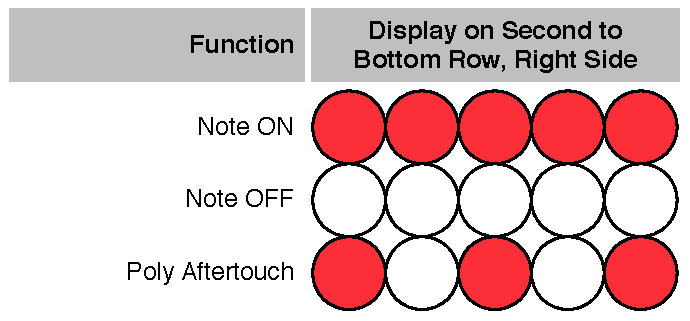
\includegraphics[width=1.6in]{notefunction.pdf}
\vspace{-2em}\caption{\small Note Function}\vspace{-2em}
\label{notefunction}
\end{wrapfigure}


Note messages are displayed with both the {\bf pitch} (at left) and the {\bf velocity} (at right) of the note value, plus the particular kind of message in question: {\bf Note On, Note Off,} and {\bf Polyphonic Aftertouch}.

\begin{wrapfigure}{r}{1.8in}
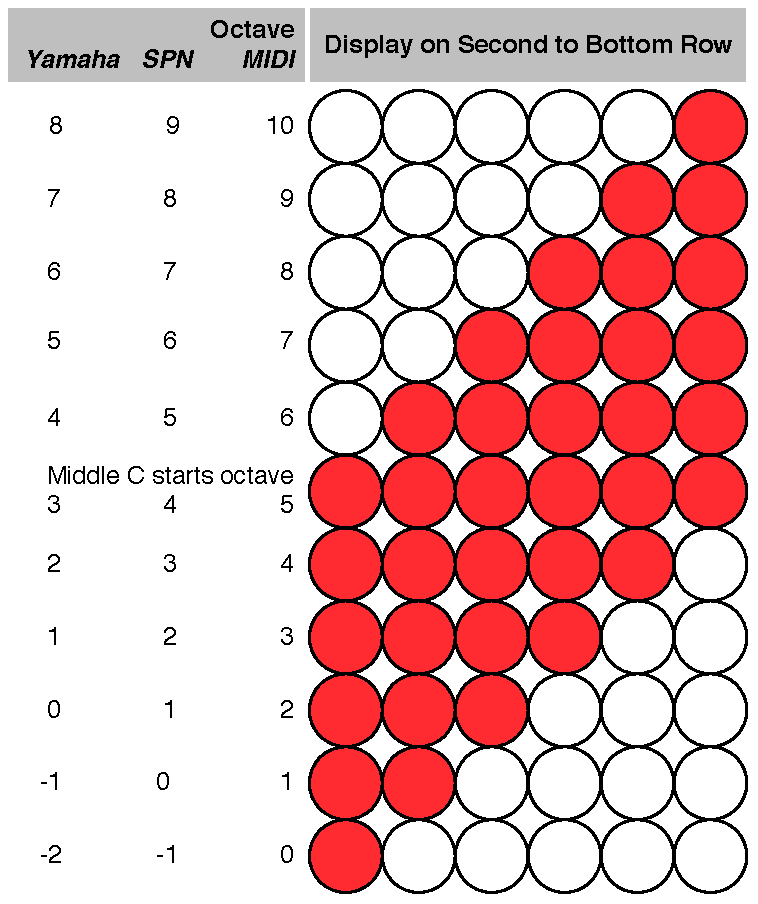
\includegraphics[width=1.8in]{octave.pdf}
\vspace{-2em}\caption{\small Octave Values.  Three common octave numbering schemes shown: Yamaha, SPN (so-called {\it Scientific Pitch Notation}), and MIDI.  SPN is the most common on keyboards.}\vspace{-5em}
\label{octave}
\end{wrapfigure}


\paragraph{Note Display}


How exactly do you distinguish between a Note On, Note Off, or Polyphonic Aftertouch message then?  Figure~{\ref{gaugedisplays}}~[Right] shows a four-LED region, in orange, where a certain pattern is displayed to indicate this.  The patterns are shown in Figure~\ref{notefunction}.

Note pitches are displayed by showing the note (such as B$\flat$), with the octave value directly below it.  MIDI has eleven different octaves (0--10): Middle C is the bottom note of octave 5.  The octave number is displayed as shown in Figure~\ref{octave}.  As usual, the MIDI In Channel is shown below that.


\paragraph{Frequent MIDI Display}  These are messages which are too fast to display usefully in most cases.  In each case, a specific LED will be toggled (see Figure~\ref{gaugedisplays}).  The messages are:

\paragraph{}\vspace{-2em}\begin{itemize}
\item {\bf Active Sensing}
\item {\bf MIDI Time Code}
\item {\bf MIDI Clock}
\end{itemize}


\section {The Controller}
\label{controller}

The Controller allows you to assign to each of two buttons and two potentiometers any NRPN, RPN, Control Change (CC), or Program Change (PC) value, or (on the Mega) Pitch Bend, Channel Aftertouch, or control voltage.  These assignments are stored in Flash memory and survive reboots and power cycling.

The Controller interacts with Bypass mode differently than other applications.  In bypass mode, the Controller passes all the incoming MIDI data to MIDI out as usual.  But it will still emit values when you press the buttons or more the knobs.  This is because it's typical that you'd want to use Controller to (for example) manipulate the VCF on an analog synthesizer while playing it via a remote keyboard.  To do this, you'd plug the keyboard into Gizmo, plug Gizmo into the synthesizer, and turn on bypass mode.

Optional control voltage is sent out one of two Digital-to-Analog Converters or DACs you may have attached, which it refers to as DAC A (I2C address 0x62) or DAC B (I2C address 0x63).\footnote{Gizmo assumes you're DACs of this kind: https:/\!/www.adafruit.com/product/935\quad These DACs can be connected via I2C, send 0--5V, and can be set to either I2C address 0x62 or 0x63.  If you need more than 5V, you'll need to wire up your own op-amp.}

	\begin{description}

	\item{\bf Go}
	
	This enters the controller proper.  Turning the left or right knobs, or pressing the Select or Middle buttons, will cause them to issue MIDI messages as assigned (below).  If you press the Back button, you can exit the controller.
	
	When you turn a knob or press a button, and the knob/button has had its control type set to something other than OFF, then the appropriate MIDI message is sent, and the value of the message is displayed as a number on-screen.  Messages are only sent if the MIDI OUT channel is something other than NO CHANNEL (See {\bf Options\(\boldsymbol\rightarrow\) Out MIDI}, in Section \ref{options}).
	
	Several protocols (NRPN, RPN, some CC) can accept 14-bit numbers, that is, values in the range 0...16383.  However Gizmo's potentiometers have a maximum resolution of 10 bits, that is, 0...1023.   The potentiometers in fact send 10 bits of data: their top 7 bits are the MSB, and their bottom 3 bits become the upper 3 bits of the LSB (the bottom 4 bits are padded with zeros).   While only the MSB is displayed on-screen, this partial LSB is being sent as well to give you a bit more control.  For control voltage, all ten bits will be mapped to 0--5V.\footnote{The DACs are actually 12-bit, but what can you do: the pots are only 10 bit.}  \ For Pitch Bend, the ten bits will be mapped to \(-8192...8191\).

	\item{\bf Left Knob} and {\bf Right Knob}\quad (\texttt{L KNOB} and \texttt{R KNOB})
	
	These submenus let you select your control type and parameter number for the left and right potentiometers.
	
	In each, you are first given the option of what kind of {\bf control type} (OFF, CC, NRPN, RPN, PC, or (on the Mega) Pitch Bend, Aftertouch, A Voltage, or B Voltage) you would like to manipulate with the left knob.  If OFF, then turning the knob will not do anything.

	After you have selected a control type, if you have selected CC, NRPN, or RPN, you will be then asked to select a {\bf controller parameter number}.  (Otherwise ,for PC and OFF, you will go back to the top-level Controller Menu).  CC parameter numbers may range 0 ... 119.  NRPN and RPN parameter numbers may range 0 ... 16383. When you have completed this, you will be sent back to the top-level Controller menu.

	\item{\bf Middle Button} and {\bf Select Button}\quad (\texttt{M BUTTON} and \texttt{R BUTTON})
	
	Thees submenus let you select your control type, parameter number, and on/off values for the middle and select buttons.
	
	In each, you are first given the option of what kind of {\bf control type} (OFF, CC, NRPN, RPN, PC, or (on the Mega) Pitch Bend, Aftertouch, A Voltage, or B Voltage) you would like to manipulate with the middle button.  If OFF, then pressing the button will not do anything.

	After you have selected a control type, if you have selected CC, NRPN, or RPN, you will be then asked to select a {\bf controller parameter number}.  (Otherwise ,for PC and OFF, you will go back to the top-level Controller Menu).  CC parameter numbers may range 0 ... 119.  NRPN and RPN parameter numbers may range 0 ... 16383.
	
	When you have completed this, you will be then asked to enter the value sent when the button is {\bf pressed}.  This value must be 0...127 (the Controller does not send 14-bit values).  Afterwards, you will be similarly asked to enter the value sent when the button is {\bf pressed again} (the buttons act as toggles).  When you have completed this, you will be sent back to the top-level Controller menu.

		\item{\bf \textit{Note}} At the borders of 14-bit values (near 0 or 16383) you may find it harder to precisely set the BPM due to anti-potentiometer noise code in Gizmo. Just use the right knob to fine-tune your value. 
	\end{description}
	
\paragraph{Warning} Gizmo could {\it theoretically} react to knob changes every 4 MIDI bytes read at full MIDI speed.  However an RPN/NRPN command will take up to 12 bytes (or 18 if \texttt{INCLUDE\_SEND\_NULL\_RPN} is turned on in the code), and a CC command could take up to 6 bytes.  This means that turning a knob may cause Gizmo to generate RPN/RPN/CC messages faster than it can send them.  Eventually the Arduino's write-buffer will fill with unwritten messages and the Arduino will pause until it's sent stuff out.  This could cause Gizmo to miss an incoming MIDI byte.  So if you're sending control commands while (say) at the same time passing data through, this may be an issue: though I have never had it happen to me.


\clearpage

\section {The Keyboard Splitter}
\label{splitter}

\begin{wrapfigure}{r}{3in}
\vspace{-1.5em}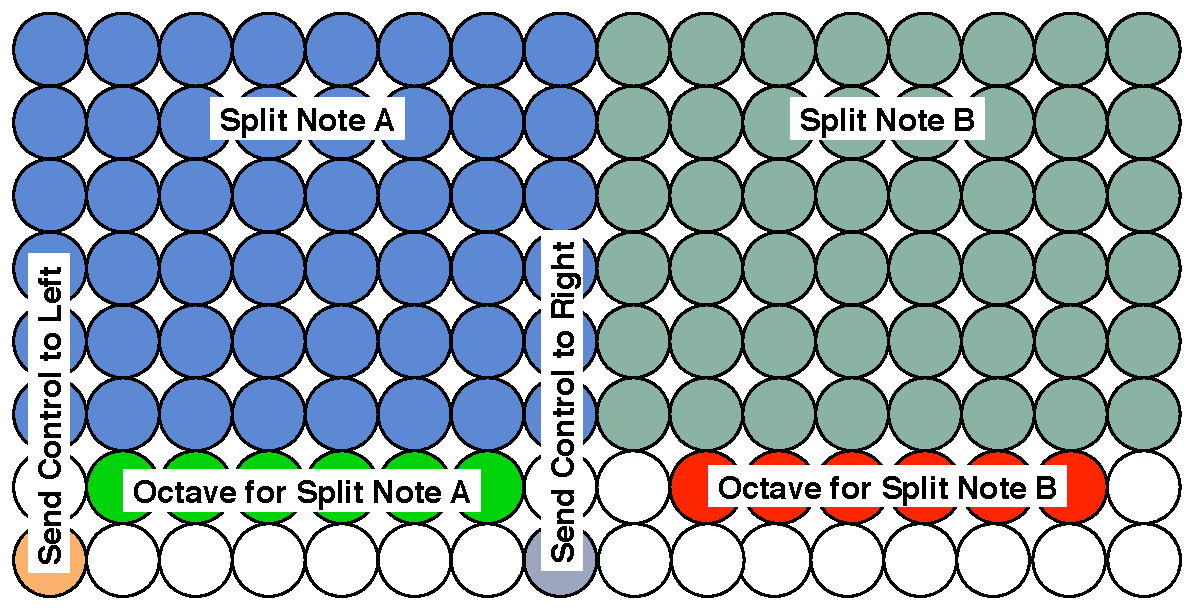
\includegraphics[width=3in]{split}
\vspace{-2em}\caption{\small Splitter Layout}
\label{splitter}
\end{wrapfigure}

\textit{[Mega Only]}\qquad The Splitter allows lets you (1) split your keyboard into two zones, each controlling a different MIDI channel; or (2) split your keyboard into {\it three} zones, two controlling different MIDI channels and the third (middle) zone playing both MIDI channels simultaneously\footnote{This is commonly known as {\it layering.}}; or (3) fade or balance your entire keyboard such that if you play a note quietly, one channel will predominate, but if you play loudly, the other channel will predominate.

The two MIDI channels in question are the Default MIDI Out Channel (defined in the Options, see Section \ref{options}), and an Alternative MIDI Out Channel which you specify in the Splitter.  If you're splitting your keyboard, you'll also specify up to two notes, {\bf Split Note A} and {\bf Split Note B}  (Split Note B is optional), and whether Control Change, Aftertouch, and the like go to the left split region or the right split region.

\begin{itemize}
\item  If you want to just split your keyboard, specify only Split Note A at the split point.  Notes in the left (lower) region will go our the Alternative MIDI Channel, and notes in the right (upper) region will go out the Default MIDI Channel.

\item If you want your keyboard to play {\bf both} channels, make Split Note A be the lowest note on your keyboard, and Split Note B be the highest note on your keyboard.    Notes played on the keyboard will be sent out both the Alternative MIDI and Default MIDI Channels. 

\item If you want your keyboard to have {\bf three regions}, a left-only region, a right-only region and a middle region where both are played, make Split Note A be the lower note in the middle region and Split Note B be the higher note.   Notes in the left (lower) region will go our the Alternative MIDI Channel, notes in the right (upper) region will go out the Default MIDI Channel, and notes in the middle region will go out both channels.

\item Note that it is possible to also give you keyboard three regions where in the middle region {\bf neither} channel is played.  This is probably not very useful.  But it happens when you define Split Note A to be {\it above} (to the right of) Split Note B.

\item Finally, if you want to fade or balance your keyboard so that notes on the two channels are played with opposite velocities, you simply choose this option (see below).  You don't need to specify either Split Note A or B, but you will need to define the alternative MIDI Channel.
\end{itemize}

\begin{wrapfigure}{r}{1.5in}
\vspace{-3em}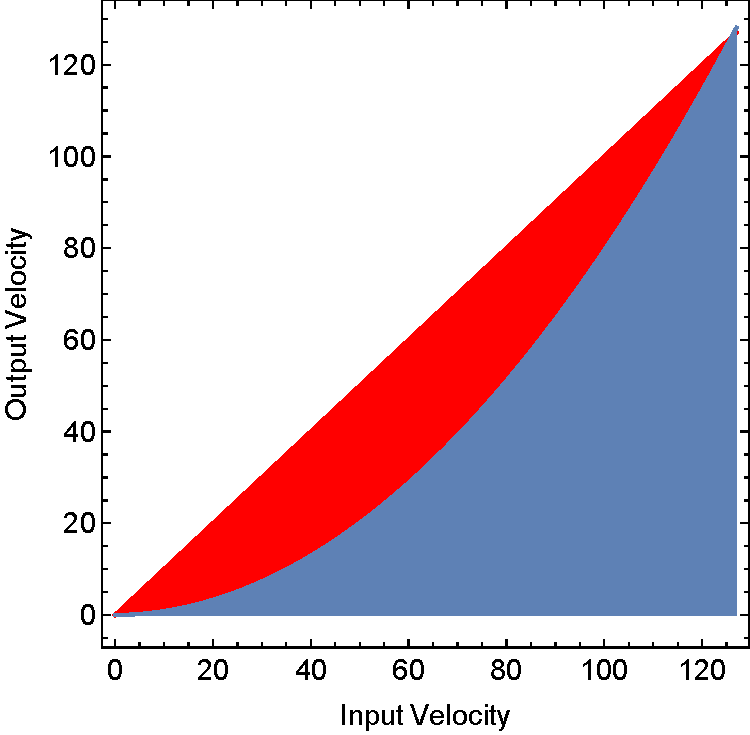
\includegraphics[width=1.5in]{Fade}
\vspace{-2em}\caption{\small Cumulative Velocity the MIDI Out Channels when fading.  Default is {\color{red}red}, and Alternative is {\color{blue} blue}.}
\vspace{-3em}
\label{splitter}
\end{wrapfigure}

\paragraph{Fade Behavior}  The current fade behavior function is:
\[
\begin{split}
\text{\it Default MIDI Velocity} &= Velocity - \text{\it Velocity} \times \left( \text{\it Velocity} + 1 \right) / 128\\
\text{\it Alternative MIDI Velocity} &= \text{\it Velocity} \times \left( \text{\it Velocity} + 1 \right) / 128
\end{split}
\]

This is a fancy way of saying that the total velocity of both channels is the same as the input velocity, and that the ratio of the Alternative velocity versus the Default velocity increases linearly as you get closer to 127.  I don't know if this is the right approach, and certainly different keyboards synthesizers have different and often nonlinear velocity mappings.  But there you have it.  If you'd like to play with it, it's in the function \texttt{handleNoteOn(...)} in \texttt{TopLevel.cpp}.

As you play notes in the fader, their velocity will appear on-screen.

\paragraph{Defining Notes and Channels}

If you press the Select Button, you'll be asked to enter a note.  This note will be Split Note A.  By default this note is Middle C.  You can back out if you don't want to enter the note.

If you press the Middle Button you'll be asked to enter a note.  This note will be Split Note B.  By default this note is off.  You can back out if you don't want to enter the note.  You can also turn Split Note B off again by once again pressing the Middle Button, at which point you'll be presented with \texttt{-~-~-~-}.  You can also back out if you don't want remove Split Note B.

\begin{wrapfigure}{r}{1in}
\vspace{-1em}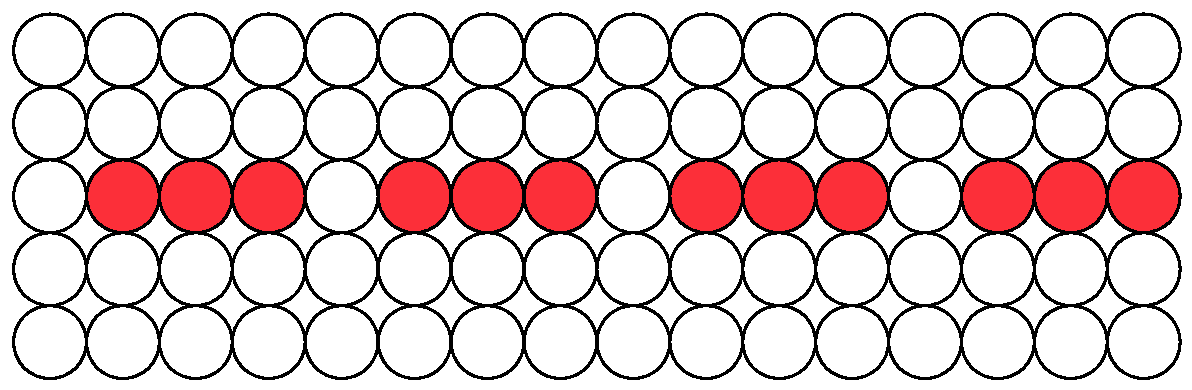
\includegraphics[width=1in]{none}
\vspace{-2em}
\end{wrapfigure}

You define the Alternative MIDI Out channel by Long-Pressing the Select Button.  The Alternative MIDI Channel must be a value 1--16 (you can't choose Off).

The Splitter will display your two Split Notes, as shown in Figure \ref{splitter}.

\paragraph{Routing and Fading}

Long-pressing the Middle Button cycles through three options:
\begin{itemize}
\item Split/Layer the Keyboard, and route all CC, PC, Channel Aftertouch, and NRPN/RPN to the {\it right} (upper) split channel, that is, to the Default MIDI Out channel.  Pitch Bend is also routed to the right channel if you're doing a simple split, but if you're layering, it's routed to both channels.  Polyphonic Aftertouch is always routed to the channel handling the note in question, as are all Note On and Note Off messages.  The screen will show the Split A note, and will light the ``left'' LED (see Figure \ref{splitter})..
\item Split/Layer the Keyboard, and route all CC, PC, Channel Aftertouch, and NRPN/RPN to the {\it left} (upper) split channel, that is, to the alternative MIDI Out Channel.  Pitch Bend is also routed to the left channel if you're doing a simple split, but if you're layering, it's routed to both channels.  Polyphonic Aftertouch is always routed to the channel handling the note in question, as are all Note On and Note Off messages.  The screen will show the Split A note at left and the Split B note at right, and will light the ``left'' LED (see Figure \ref{splitter}).
\item Fade/Balance the Keyboard.  CC, PC, Channel Aftertouch, and NRPN/RPN is routed to the alternative MIDI Out Channel.  Pitch Bend, Polyphonic Aftertouch, all Note On and Note Off messages (though with inverted velocities as discussed earlier) are routed to both channels.  The screen will display \texttt{FADE}.
\end{itemize}


\begin{figure}[h!]
\vspace{-1em}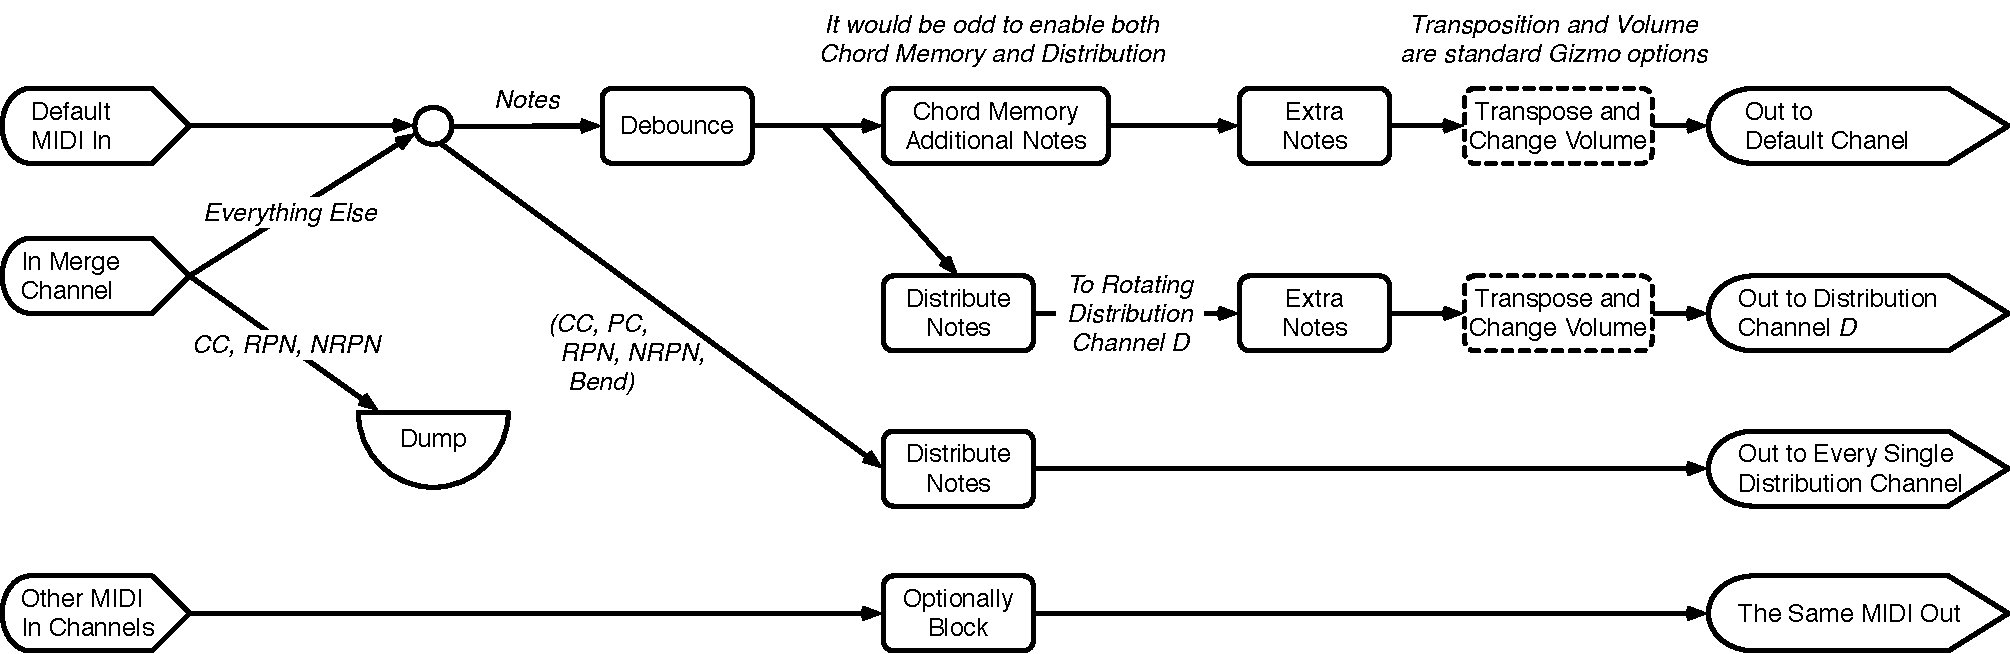
\includegraphics[width=6.5in]{thru.pdf}
\vspace{-1.25em}
\caption{Flow graph of the Thru Facility.}
\vspace{-0.5em}
\end{figure}

\section{The Thru Facility}
\label{thru}

\textit{[Mega Only]}\qquad The {\bf Thru Facility} passes MIDI through the box, but if MIDI data comes in via certain channels, it applies various optional transformations to it before it sends it out:

\begin{itemize}
\item First, you can {\it merge} two incoming channels: the Default MIDI In channel and a {\bf Merge Channel}.  Additionally you can also merge {\it all} channels by simply setting the Default MIDI In channel to OMNI.  Additionally, channels other than Default MIDI and Merge are passed through, unless you {\it block} them.

\item Note data and Control data (CC/PC/RPN/NRPN/Pitch Bend) are then handled differently. We'll start with Note data.   Note data is passed through an option that allows you to {\bf debounce notes}.   The objective here is to counteract the situation where you hit a drum pad, and instead of staying down, it quickly bounces up, then down again, resulting in a buh-dum sound..\footnote{For example, I have debouncing issues with the Arturia Beatstep.}  It works like this.  When you first press a note, Gizmo will require that this note be no less than \(N\) milliseconds long.  Furthermore, if the same note is pressed within these \(N\) milliseconds, Gizmo will ignore it.     Large values of \(N\) catch more bounces but prevent you from playing the pad rapidly, and will also prevent you from making short stabs.  Thus this would be better for one-shot sounds (drums, etc.) which play in their entirety regardless of when the note-off occurs.

\item You can then {\bf distribute} incoming notes, one by one, to separate MIDI channels, rotating the distribution round-robin.  Thus if you have multiple copies of the same monosynth, you could distribute notes to the various synths and basically treat them as if they were a polysynth.\footnote{This is an idea directly stolen from the MIDIPal.}

\item Further, you can have Gizmo add {\bf extra notes}, that is, pile up notes you're playing multiple times extremely rapidly.  For example, if you play the note G, Gizmo might send four G notes out essentially at the same time.  This is useful for fattening up a synth but not making it fully unison (mono).  For example, I have an Oberheim Matrix 1000 with six voices.  If I instruct Gizmo to provide two extra notes, then every time I press a note, Gizmo emits {\it three} copies of that note to the Oberheim, causing three voices to play together.  This basically turns the Matrix into a fatter two-voice polysynth.  {\bf Important Note}: Polyphonic Aftertouch is not repeated.\footnote{\label{serialbuffer}Because it overwhelms the Arduino's serial output, which blocks, causing Gizmo to miss messages, resulting in stuck notes.}

\item You can also perform {\bf chord memory}.  Here you first specify a chord, and then afterwards, every time you play a note, Gizmo will instead emit that chord, transposed so that its lowest note corresponds with the note you played.  This is a classic facility available on a number of synthesizers, including early ones such as the Oberheim OB-Xa, Sequential Circuits Prophet 600, Korg PolySix, and so on.\footnote{This idea was also directly stolen from the MIDIPal.}   {\bf Important Note}: Polyphonic Aftertouch is not chorded.\footnote{See Footnote \ref{serialbuffer}.}

\item Control Data (CC/PC/RPN/NRPN/Pitch Bend) follows a different path: a copy is sent to every channel that Gizmo is presently distributing to.  
%First, you're given the option of {\bf mapping CC to NRPN Data}.  Some devices (for example, the Matrix 1000 with 1.20 ROM) expect NRPN, but few DAWs (grrr) send NRPN; furthermore, most DAWs send raw CC values in total violation of MIDI spec.  At present Gizmo can convert all 128 raw CC numbers to their equivalent NRPN parameter numbers.

\item CC/RPN/NRPN from the Merge Channel is neither merged nor passed through, but is simply ignored.  This is because it is nontrivial to merge it.

\item Data from channels other than Default MIDI In and Merge is simply passed through.  {\bf Warning.}  If your Default MIDI Out is not the same as your Default MIDI In (that is, you're routing from one channel to another) 

\item Finally, if you are distributing incoming notes, control data will also be {\bf distributed}, but instead of sending it round-robin to each of the relevant channels, control data is sent to {\bf all of them in parallel}.

\end{itemize}

I might add more unusual transformers later.  Anyway, here are your options:

	\begin{description}
	
	\item{\bf Go}\\
		Once you have set up your Thru options (see below), if you choose {\bf Go}, the Thru facility starts and you can start playing.  You'll see the word \texttt{PLAY} on the LED.

	\item{\bf Extra Notes}\\
		This lets you select how many {\it additional} simultaneous note-on (and note-off) messages Gizmo should send down a given channel in response to you playing a note.
		\begin{description}
		\item{\bf \textit{Choose}}: No Extra Notes, or 1...31 \hspace{3in}\smash{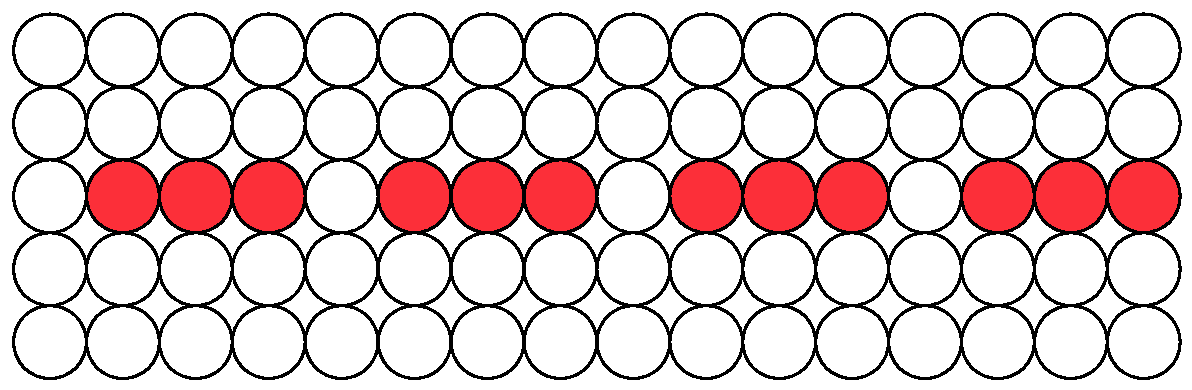
\includegraphics[width=1in]{none.pdf}} 
		\end{description}

	\item{\bf Distribute Notes}\\
		This lets you select the number of MIDI channels, beyond the Default MIDI Out channel, over which to distribute notes.  Let's say you selected 2, and the Default MIDI Out channel was \(M\).  This means that three MIDI channels will be used: \(M\), \(M+1\), and \(M+2\).  This wraps around: if, say, \(M = 15\), then it wraps around: the channels used would be 15, 16, and 1).
		
		If you played the five notes A, B, C, D, E, Gizmo would send A down channel \(M\), then send B down channel \(M + 1\), then send C down channel \(M + 2\), then send D down channel \(M\) again (wrapping around), then E down channel \(M+1\) again, and so on.  This would let you essentially use Mono devices listening in on the three MIDI Channels as a 3-voice polyphonic device.
		
		\begin{description}
		\item{\bf \textit{Choose}}: No Extra Channels, or 1...15 \hspace{2.8in}\smash{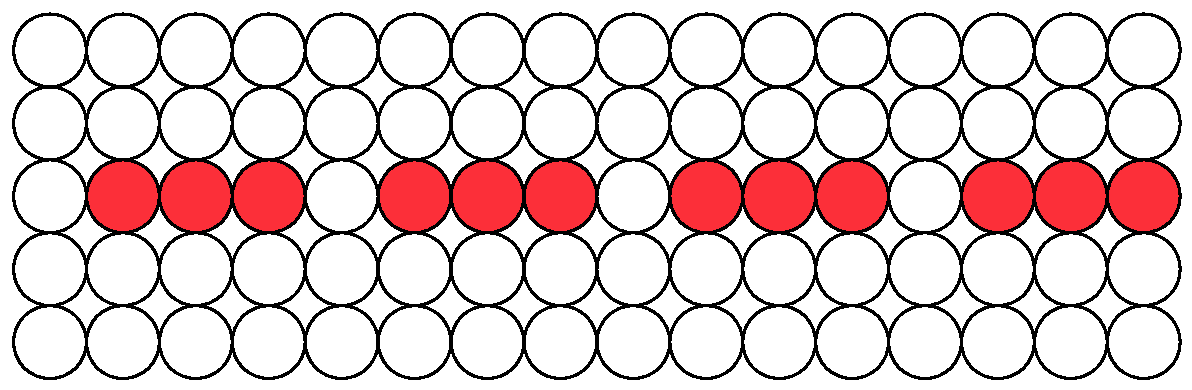
\includegraphics[width=1in]{none.pdf}} 
		\end{description}

	\item{\bf Chord Memory} or {\bf No Chord Memory}\\
		This will show the text \texttt{CHRD}, and you can then specify a chord (of up to eight notes).  Thereafter if you play a single note, the chord will be played instead, transposed so that its root note corresponds with the note you play. (If you play more than one note, more than one chord will be played).  If you have already chosen a chord, then selecting this option again will turn off chord memory.
				
		\begin{description}
		\item{\bf \textit{Choose}}: a chord of up to eight notes.
		\end{description}
		
	\item{\bf Debounce}\\
		This lets you choose the number of milliseconds between successive identical MIDI notes (the \(N\) value discussed earlier).  100 milliseconds seems to work well for me.
		\begin{description}
		\item{\bf \textit{Choose}}: No Debouncing, or 1...255 (milliseconds)\\\rule[0em]{0em}{0em}\hspace{\fill}\smash{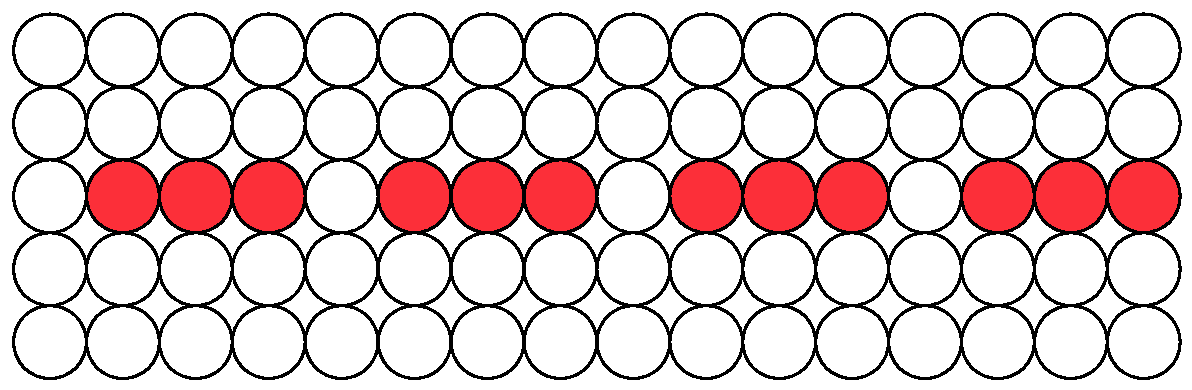
\includegraphics[width=1in]{none.pdf}} 
		\end{description}

	\item{\bf Merge Channel}\\
		Here you select the alternate MIDI-In channel (if any) to merge with the Default MIDI In channel
		\begin{description}
		\item{\bf \textit{Choose}}: No Channel, Channels 1...16, or ALL Channels (OMNI)\hspace{0.25in}{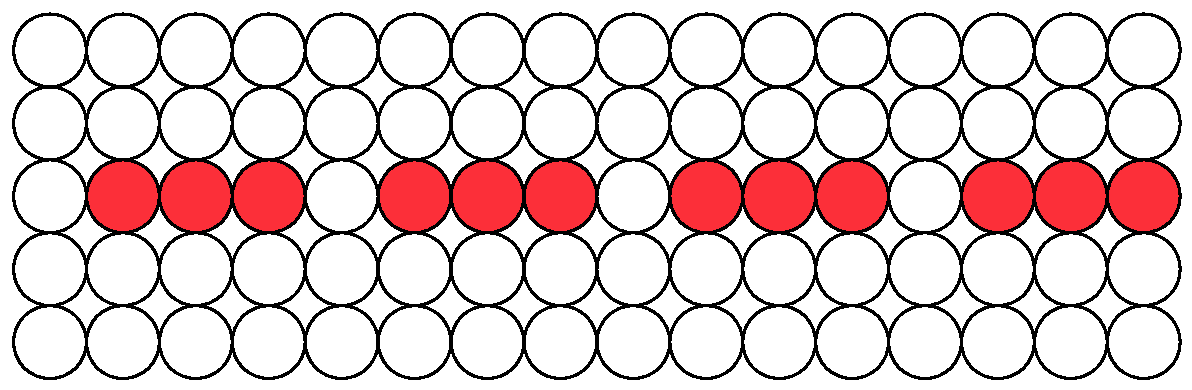
\includegraphics[width=1in]{none.pdf}}~{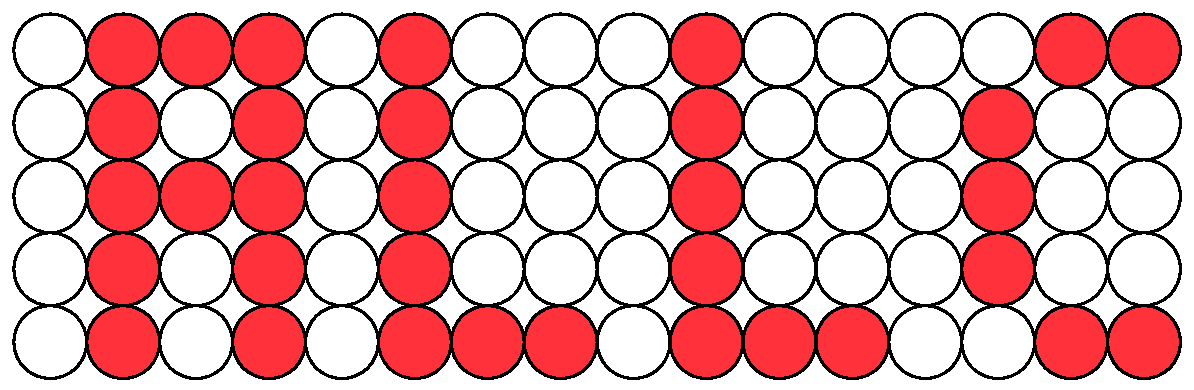
\includegraphics[width=1in]{all.pdf}}
		\end{description}

%	\item{\bf CC-NRPN} or {\bf No CC-NRPN}\\
%		This will toggle whether raw CC is converted to equivalent NRPN values.
				
	\end{description}

\section {Synthesizer MIDI Helpers}
\label{synthesizer}

\textit{[Mega Only]} Synthesizers often have weak spots in their MIDI implementations.  This application contains various submenus, one per synthesizer, designed to provide an assist for that particular model.\footnote{Why {\it these particular models?}  Because I own them. If you'd like me to write a helper for another machine here, send me a synth!}

\paragraph{A Note on Performance} Often these MIDI helpers are converting CC to NRPN, or converting NRPN to Sysex, and in the process they're emitting something bigger than they're getting (for example, an NRPN message could be between 3 and 5 times larger than a CC message).  This is a problem.  For example, if it receives CC at a very fast rate, Gizmo won't be able to send out corresponding NRPN fast enough and eventually Gizmo's serial input buffer will overflow.  To counter this, Gizmo sends out messages at a fixed rate (typically about 100 per second), and drops some on purpose if they arrive faster than that.   Gizmo will always send the most recent packet.  This is determined by some constant \texttt{\textit{SYNTH\_NAME}\_COUNTDOWN} in the appropriate file \texttt{synth/\textit{SynthName}.h} (lower values are faster rates).


\subsection{Waldorf Blofeld Module / Keyboard}  The Blofeld exposes parameters through CC, not NRPN; this means that not all of its parameters can be accessed (there too many of them).  Gizmo maps NRPN messages to corresponding Blofeld Sysex parameter change messages, which allows you to manipulate all of the Blofeld's parameters over NRPN.  The NRPN parameter numbers in question are 0...382 (MSB + LSB), corresponding to the Sysex parameters shown in Section 3.1 (``SDATA - Sound Data'') of the text file found in \texttt{docs/synth/WaldorfBlofeldSysex.txt} in the Gizmo distribution.  Values are MSB only.  Additionally, changing the value of NRPN parameter number 400 will set the buffer which these parameters effect, namely, 0 (Sound Mode Edit Buffer or Multi Instrument Edit Buffer 0), or 1--15 (Multi Instrument Edit Buffers 1...15).  The default is 0.

\paragraph{Display}  If you are setting the ID, then \texttt{ID} is displayed, along with the ID value.  Otherwise, just the set value is displayed.

\paragraph{Caveats} While you are sending NRPN this way, you can also send some CC messages, but not for CC numbers 6, 32--63, or 98--101: you'll need to send the NRPN equivalents for those.  The Blofeld seems to drop some Sysex packets if you send them too fast.  Significantly increasing \texttt{WALDORF\_BLOFELD\_COUNTDOWN} helps things but at the cost of lag and discretization.  It's probably better to just turn your encoder dial more slowly.

\subsection{Kawai K4 / K4r}  {\color{red} This code is not yet tested}\quad The K4 is only accessible via Sysex.  Gizmo maps NRPN messages to corresponding Kawai K4 Sysex parameter change messages, which allows you to tweak all of the K4's (non-Multi) parameters over NRPN.  The K4 has 88 parameters, broken into Single (0--69), Drum (70--81), and Effect (82--88) parameters.  Single parameters require that you first specify the {\it source} via NRPN parameter 100: source 1 is value 0, source 2 is value 1, source 3 is value 2, and source 4 is value 3.  Drum parameters require that you first specify the {\it drum key} via NRPN parameter 101: the key values are 0--60, left to right.  And Effect parameters require that you first specify the {\it submix / output channel} via NRPN parameter 101: channel values are 0--7.  

For more information, see the PDF file \texttt{docs/synth/KawaiK4CorrectedMIDIImplementation.pdf}.  In particular, look at to the breakout of parameters as specified in Section 5-6 and the parameter list proper in Section 6 (pay attention to the ``Parameter No'' column).   Note that one parameter (\#17) combines four mute values and vibrato shape into a single number.  This means you can't change one of them without changing the others.  Gizmo handles this by letting you set each of them separately, and it keeps track of what settings you used previously.  Set all of them one time each, then as you continue to set them it'll update with the old values of the others.  Mutes 1--4 are set with NRPN parameter 103--106, and Vibrato Shape is set with NRPN parameter 107.  See Parameter \#17 in Section 6 of the file for appropriate values of these.

\paragraph{Display}  If you are setting the Vibrato Shape or Mute 1...4, then \texttt{VS}, \texttt{M1}, \texttt{M2}, \texttt{M3}, or \texttt{M4} are displayed respectively, along with the value.  If you are setting the Source, Drum, or Effects Parameter, then \texttt{S}, \texttt{D}, or \texttt{FX} are displayed respectively along with the value.  Otherwise, just the value is displayed.


\subsection{Oberheim Matrix 1000}  {\color{red} This code is not yet tested}\quad This machine is dramatically opened up by new firmware (Gligli's v1.16, and Bob Grieb's v1.20), which adds quasi-real-time parameter changes and NRPN support.  If you don't have this firmware yet, you should install it.\footnote{I strongly suggest you install Bob Grieb's, it's only \$30.  http:/\!/tauntek.com/Matrix1000Firmware.htm\quad By the way, if you have a Matrix 6 or 6R, check out http:/\!/tauntek.com/Matrix6Firmware.htm though it doesn't support NRPN.}  Unfortunately few DAWs support NRPN.  So Gizmo lets you map raw CC messages to their NRPN counterparts.  The mapping work as follows.  The Matrix 1000 has parameters 0--99.  To send the Matrix 1000 an NRPN parameter \(p\) from 0--53, you send a CC parameter of \(p+10\) (so this ranges 10--63).  To send an NRPN parameter \(p\) from 54--99, you send a CC parameter of \(p+20\) (so this ranges 74--119).  If you send a CC parameter 0--10, 64--73, or 120--127, it is passed through as a regular CC message.  To understand the 99 (actually somewhat fewer) parameters, find an online copy of the Matrix 6 ({\it not} Matrix 1000) manual.\footnote{You can also see the parameter list and MIDI implementation at http:/\!/www.youngmonkey.ca/nose/audio\_tech/synth/Oberheim-Matrix1000.html\quad Pay attention to the section ``MATRIX-1000 SINGLE PATCH DATA FORMAT'', particularly the ``Parameter'' column.}  Also note that because many Matrix 1000 parameter values are signed (such as -64...63), the NRPN values are implemented unsigned (0...127) in the machine as follows.  To send a value \(v\), you should instead send \(v+64\).  For example, to send 15, you should actually send 15 + 64 = 79, and to send -3, you would send -3 + 64 = 61.  One exception: for parameter number 21 (VCF Initial Frequency), you should just send the number as-is.

\paragraph{Display} Just the set value is displayed.


\subsection{Korg Microsampler}  Anyone who owns one of these machines knows that its MIDI is a disaster.  Pitch Bend is steppy, only certain notes can be played, if MIDI START is received the pattern sequencer immediately starts up, and if the device is set to emit MIDI clock (via ``auto'' or ``internal'') then MIDI clock pulses are sent but not MIDI START, STOP, or CONTINUE.  These last two items can be overcome with judicious use of Gizmo's MIDI clock filter.  But on top of it all, the Microsampler's parameters can only be controlled via sysex,\footnote{And not all of them: you can't change the start or end trim positions, for example.  Furthermore, no {\it events} can be controlled by sysex.  So there's no sysex message to tell the Microsampler to start recording, or to normalize the sound.} and it's entirely undocumented. 

Gizmo's helper for the Microsampler converts NRPN to sysex.  There are four basic kinds of parameters.  First there are {\it bank parameters}, such as BPM.  These are changed straightforwardly with one NRPN command each.  Second, there are {\it pattern parameters} such as Pattern Length.  These require a pattern number in addition to the parameter number.  To change these, you either first set the pattern number \(n\) via NRPN 50 and then set the parameter via its NRPN \(p\), or you can change the parameter  directly by changing NRPN number \(p + 100 \times n\).  Third there are {\it sample parameters} such as Sample Level.  Similar to pattern parameters, these require a sample number in addition to the parameter number, and similarly, you can either first set the sample number \(n\) via NRPN 51 and then set the parameter via its NRPN \(p\), or you an change the parameter directly by changing NRPN number \(p + 100 \times n\).  

Finally, there are {\it FX parameters}.  These require not two but {\it three} variables: the FX type, the FX Parameter Number, and the parameter value proper.  To set these, you first set the FX Type (NRPN 31).  This switches the FX Type on the machine.  Then you either set the FX parameter number \(n\) via NRPN 52 and then set the parameter via its NRPN \(p\), or you can change the parameter directly by changing NRPN number \(p + 100 \times n\).  Note that the number of FX parameters varies depending on the FX type chosen.

The FX type can be set independently, as can the parameters emitted by Control 1 and Control 2 (via NRPN 32 and 33 respectively).  Note that the parameters emitted by these are a subset of possible parameters for a given FX type.

The full sysex documentation to the best of my understanding, plus the Gizmo NRPN parameter mapping, can be found in the file \texttt{docs/synth/KorgMicrosamplerSysex.txt}.


\paragraph{Display} If you are setting the Sample Number, Pattern Number, or Effects Parameter Number, then \texttt{S}, \texttt{P}, or \texttt{FX} are displayed respectively, plus the number.  Otherwise only the set value is displayed.

\subsection{Yamaha TX81Z} {\color{red} This code is not yet tested, and has known bugs}\quad The TX81Z's parameters can only be changed via sysex.  Gizmo maps NRPN messages to corresponding TX81Z Sysex parameter change messages, which allows you to tweak all of them over NRPN.   One oddity in Yamaha's Sysex is that it has MIDI channels.  Gizmo will set this channel to Gizmo's MIDI Out channel.

The TX81Z has a great many parameters, split into nine different categories, each assigned a number \(c\) as shown:  (0) {\it VCED,} (1) {\it ACED,} (2) {\it PCED,}  (3) {\it Remote Switch,}  (4) {\it Octave Micro Tuning,} (5) {\it Full Micro Tuning},  (6) {\it Program Change Table,} (7) {\it System Data,} and (8) {\it Effect Data}.  In all cases, to set a parameter number \(p\) from a given category~\(c\), you choose NRPN number (MSB+LSB) \(c \times 200 + p\). The parameter numbers for categories VCED, ACED, PCED, and Remote Switch are shown on pages 71--73 of the file \texttt{docs/synth/YamahaTX81ZManual.pdf}.   System Data and Effect Data are set similarly, but the meaning of the parameters is unknown to me.  Values are 7-bit (MSB) only.

For Octave and Full Micro Tuning, the parameter number \(p\) is the key number.  The value of this number is 14-bit (MSB+LSB), where the MSB is the note to assign the key and the LSB is a fine-tuning of the note.  Gizmo deviates from the TX81Z standard here to make programming easier: the fine-tuning ranges from 1...63, where 1 is \(-31\), 32 is 0, and 63 is +31.

Because the TX81Z has more than 128 patches, Program Change Table lets you (weirdly) map PC commands (0--127) to specific patches (0--184).  See page 68 of the file for information on how these 185 patches are organized.  In NRPN, the parameter number \(p\) specifies the program change number, and the value (MSB+LSB) is the patch number.

\paragraph{Display} Just the set value is displayed.

\paragraph{Caveats}  The TX81Z doesn't respond well to fast parameter changes.    Significantly increasing the value of \texttt{YAMAHA\_TX81Z\_COUNTDOWN} may help this but at the cost of lag and discretization.  It's probably better to just turn your encoder dial more slowly.


\clearpage

\section {The Measure Counter}
\label{measure}

\begin{wrapfigure}{r}{3in}
\vspace{-1.5em}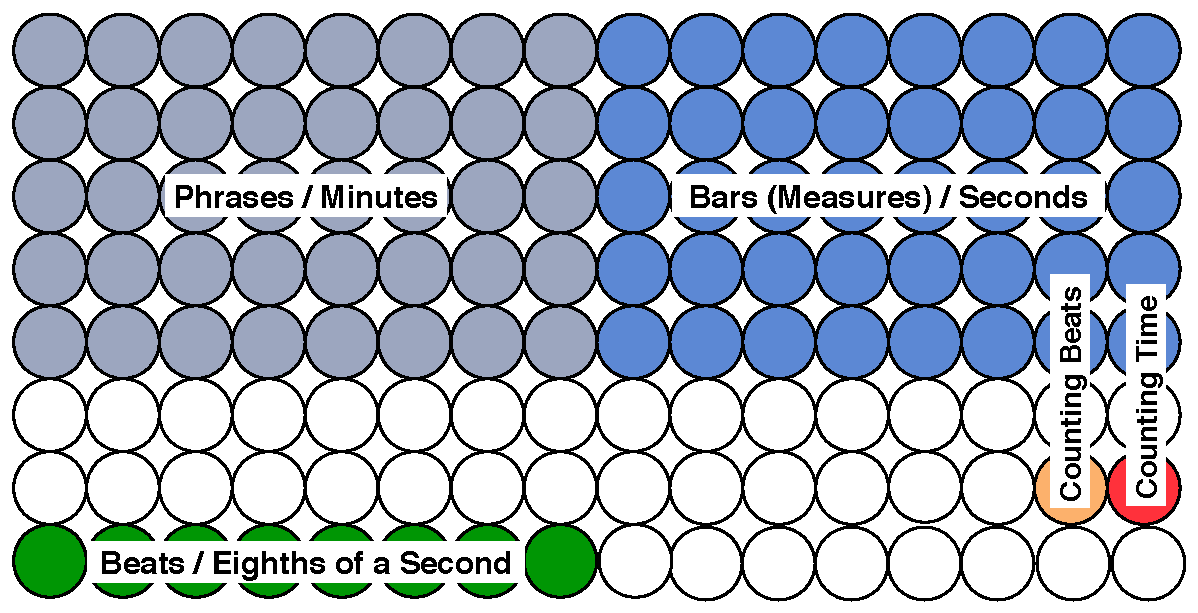
\includegraphics[width=3in]{measure}
\vspace{-2em}\caption{\small Measure Counter Layout}
\vspace{-1em}\label{measurecounter}
\end{wrapfigure}

	The measure counter\footnote{The Measure Counter was added to Gizmo at the request of \texttt{Inkog}, a member of http:/\!/gearslutz.com and early adopter of Gizmo.} is basically a stopwatch which counts elapsed beats, measures (bars), and phrases (up to 127 phrases).  Alternatively if can count eighths of a second,\footnote{\label{footnotetenths}Why not tenths of a second?  Because \(10 \times 60 \times 128\) is larger than \(2^{16}\), so it won't fit in a 16-bit integer.} seconds, and minutes (up to 127 minutes) via the internal clock or external MIDI clock.  If the minutes or phrases exceed 127, then \texttt{HI} is displayed instead.
	
	To change what a measure (bar) or phrase means, long-press the Select button to bring up the Menu.  Here you can choose the {\bf Beats Per Bar} (a value from 1...16)\footnote{Why not 32, like Bars Per Phrase uses?  Because \(32 \times 32 \times 128 > 2^{16}\).  So basically for the same reason as Footnote \ref{footnotetenths}.} and the {\bf Bars per Phrase} (1...32), and as usual, call up the {\bf Options Menu} to change the {\bf Tempo}, etc.
	
\begin{wrapfigure}{r}{2in}
\vspace{-1em}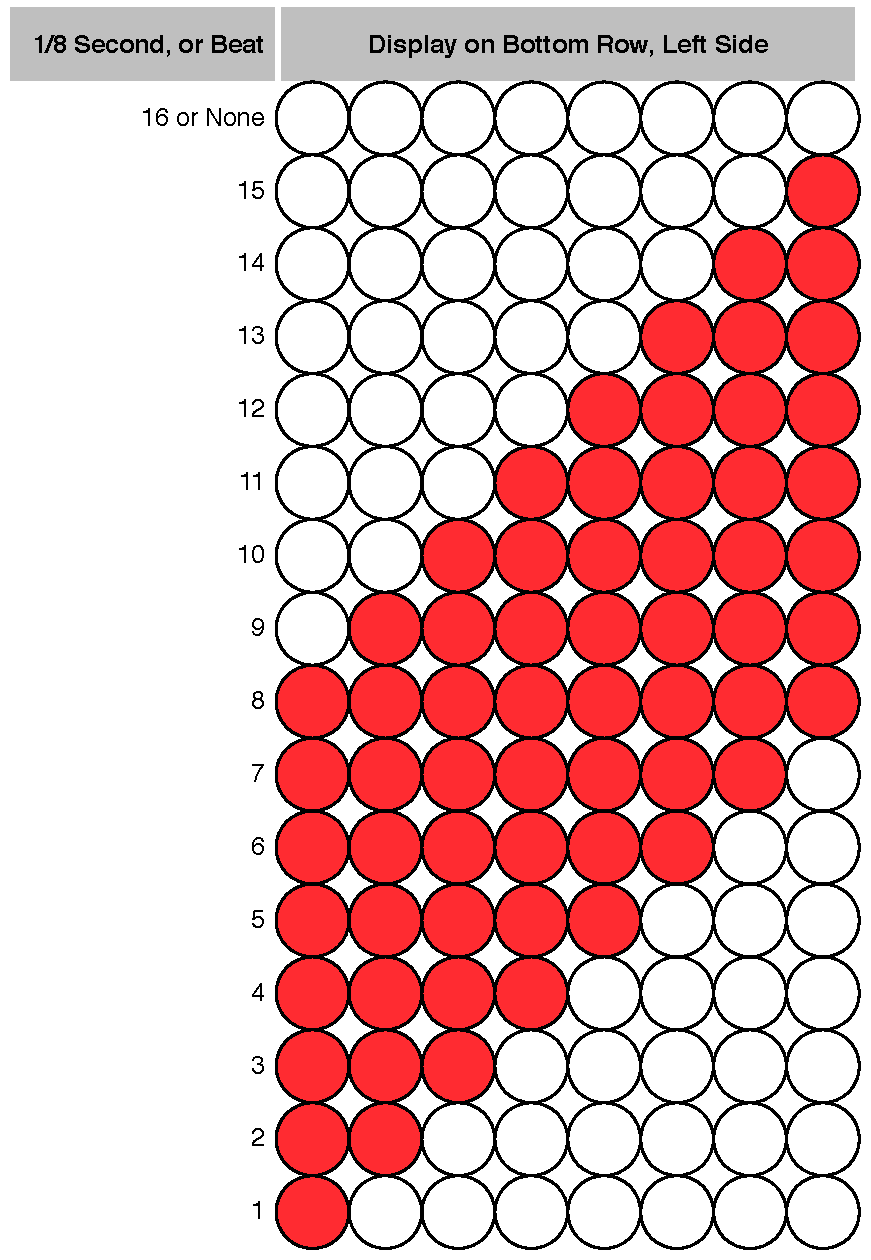
\includegraphics[width=2in]{measurebeats}
\vspace{-2em}\caption{\small Beats or 1/8 Second Ticks}\vspace{-3em}
\label{midichannelvalues}
\end{wrapfigure}


	Pressing the Middle Button starts and and restarts the stopwatch.  Long-pressing the Middle Button pauses the stopwatch (pressing the Middle Button afterwards will continue).  Additionally, external MIDI Start, Stop, and Continue commands will affect the stopwatch: Stop will pause it, Continue will continue from last pause, and Start will reset the stopwatch and start it fresh.

	Normally the measure counter shows beats, measures, and phrases.  But if you press the Select button, Measure will instead start displaying elapsed time, so it's basically a stopwatch.  More specifically, rather than counting beats, measures (bars), and phrases, Measure will count eighths of a second, seconds, and minutes.  The response to buttons is the same, as is the response to MIDI clock directives.

	You can also control the Measure Counter via MIDI: if you send a MIDI Play, it will reset the Measure Counter.  Note that if you send a MIDI Stop, and Gizmo is listening to external MIDI clock, then the Measure Counter will be halted (and MIDI Continue will continue the Counter).  However sending a MIDI Stop will not presently halt the stopwatch.

		
\section {Options}
\label{options}

	Options sets global parameters for the device.  These parameters are stored in Flash memory and survive a power cycle.  Some options can be also accessed from certain other applications as a convenience.  
	
	\begin{description}


	\item{\bf Tempo}\\
	If Gizmo is following its own internal clock rather than relying on an external MIDI clock , this specifies how fast a quarter note is.  (See {\bf Options\(\boldsymbol\rightarrow\)MIDI~Clock}).  When not in {\bf Bypass Mode}, the tempo is shown by the pulsing on/off of the {\bf Beat / Bypass Light} (see Figure~\ref{HighLevelGizmoLayout}). 
	
\begin{description}
		\item{\bf \textit{Choose}}: 1 ... 999 Beats Per Minute.  Note that this is a large number, and so may require you to choose it with the left potentiometer, then fine-tune it with the right potentiometer.\footnote{Gizmo can go lots faster than 999: in theory it could go clear to 31200 or so.  But then your synthesizer would explode and we wouldn't want that.}
		\item{\bf \textit{Alternatively}}: Tap the Middle Button.  The BPM will be set to the rate you tap.
   		\item{\bf \textit{Note}} At the borders (near 1 or 999) you may find it harder to precisely set the BPM due to anti-potentiometer noise code in Gizmo. Just use the right knob to fine-tune your value. 
		\end{description}
		
	\item{\bf Note Speed}\\
		Various applications (arpeggiators, step sequencers)
		produce notes at a certain rate relative to the tempo.
		For example, though the tempo may specify that a
		quarter note is set to 120 Beats Per Minute, the 
		arpeggiator might be generating eighth notes and
		so is producing notes at twice that speed.  You specify the 
		note speed here.
		
		Note speed is shown by pulsing the {\bf Note Pulse Light} (Figure~\ref{HighLevelGizmoLayout}).

\vbox{		\begin{description}
			\item{\bf \textit{Choose}}:
			\begin{tabbing}
			Eighth Triplet (Triplet 64th Note)\hspace{3em}\=\(\myfrac{1}{24}\)\hspace{1em}\=Beat\\
			Quarter Triplet (Triplet 32nd Note)\>\(\myfrac{1}{12}\)\>Beat\\
			Thirty-Second Note\>\(\myfrac{1}{8}\)\>Beat\hspace{0.7in}\=\smash{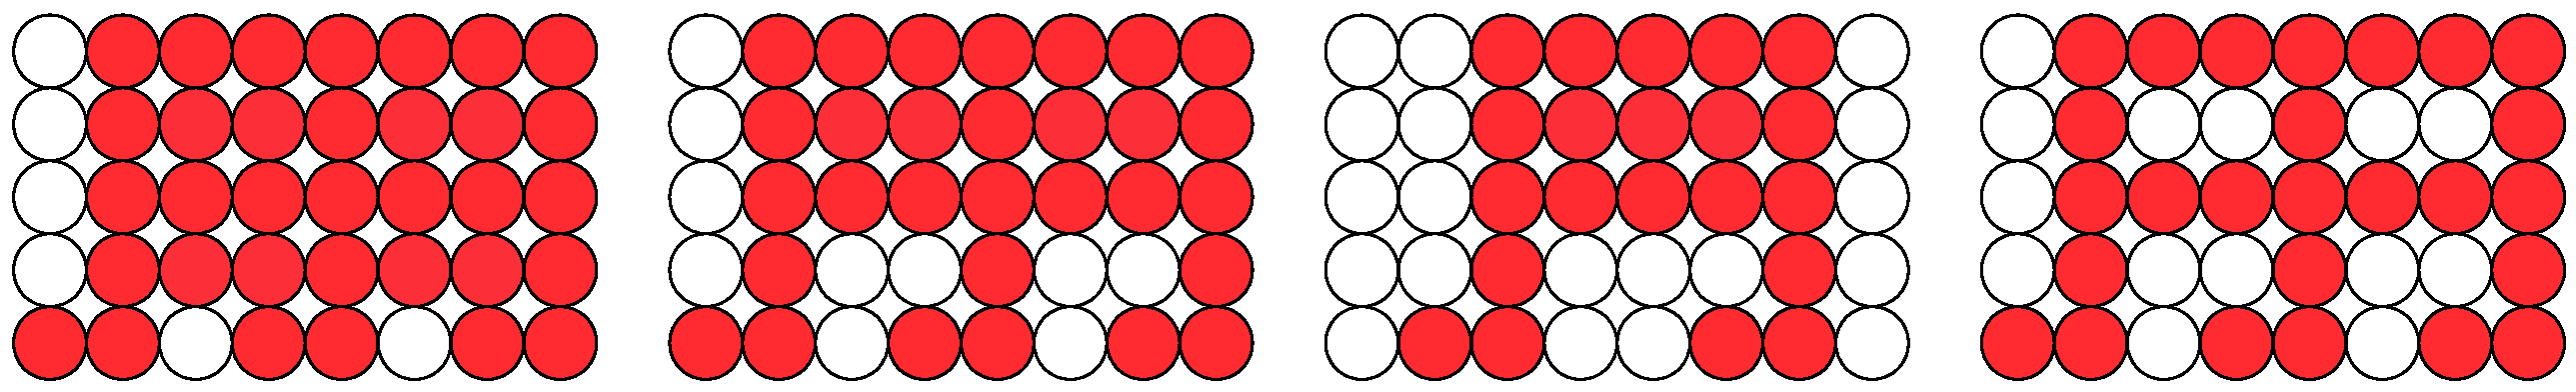
\includegraphics[width=2in]{NoteSpeed1.pdf}}\\
			Half Triplet (Triplet 16th Note)\>\(\myfrac{1}{6}\)\>Beat\\
			\\
			Sixteenth Note\>\(\myfrac{1}{4}\)\>Beat\\
			Triplet\>\(\myfrac{1}{3}\)\>Beat\\
			Eighth Note\>\(\myfrac{1}{2}\)\>Beat\>\smash{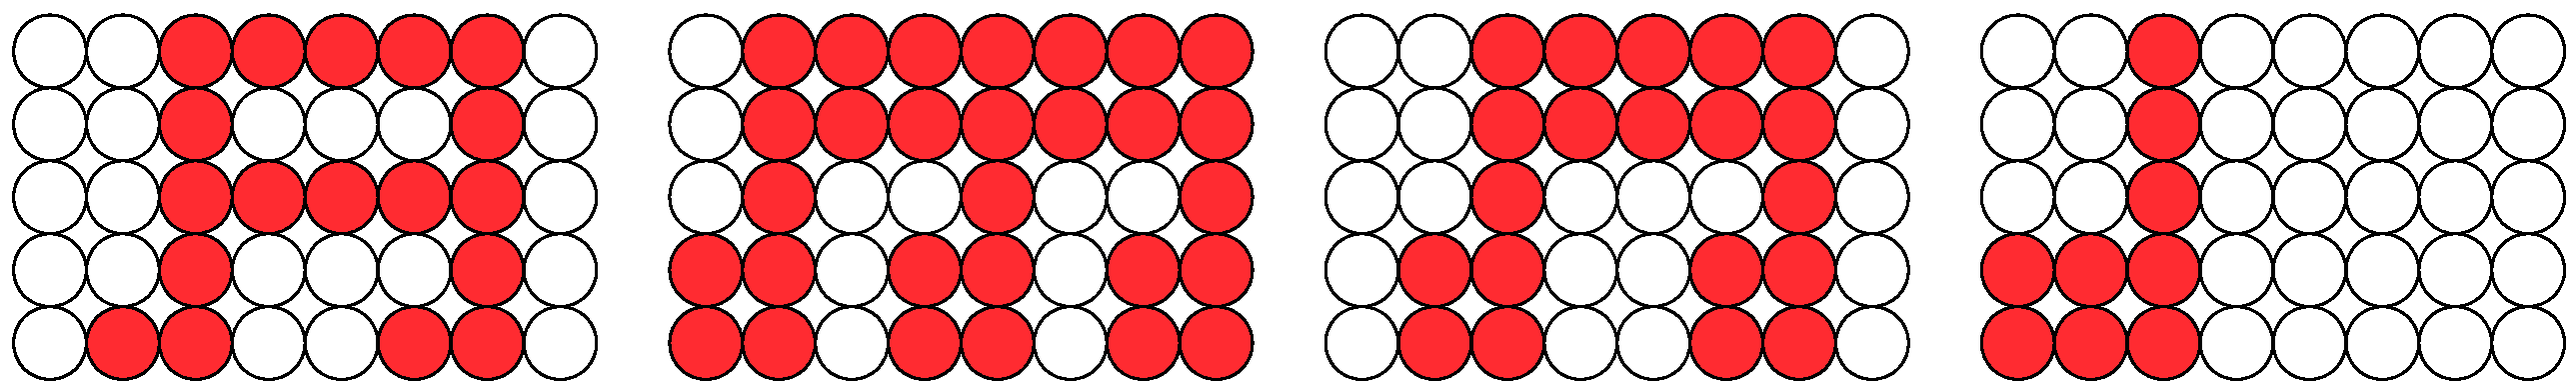
\includegraphics[width=2in]{NoteSpeed2.pdf}}\\
			Quarter Note\>\(1\)\>Beat (duh)\\
			\\
			Quarter Note Tied to Triplet\>\(1\ \, \myfrac{1}{3}\)\>Beats\\
			Dotted Quarter Note\>\(1\ \, \myfrac{1}{2}\)\>Beats\\
			Half Note\>\(2\)\>Beats\>\smash{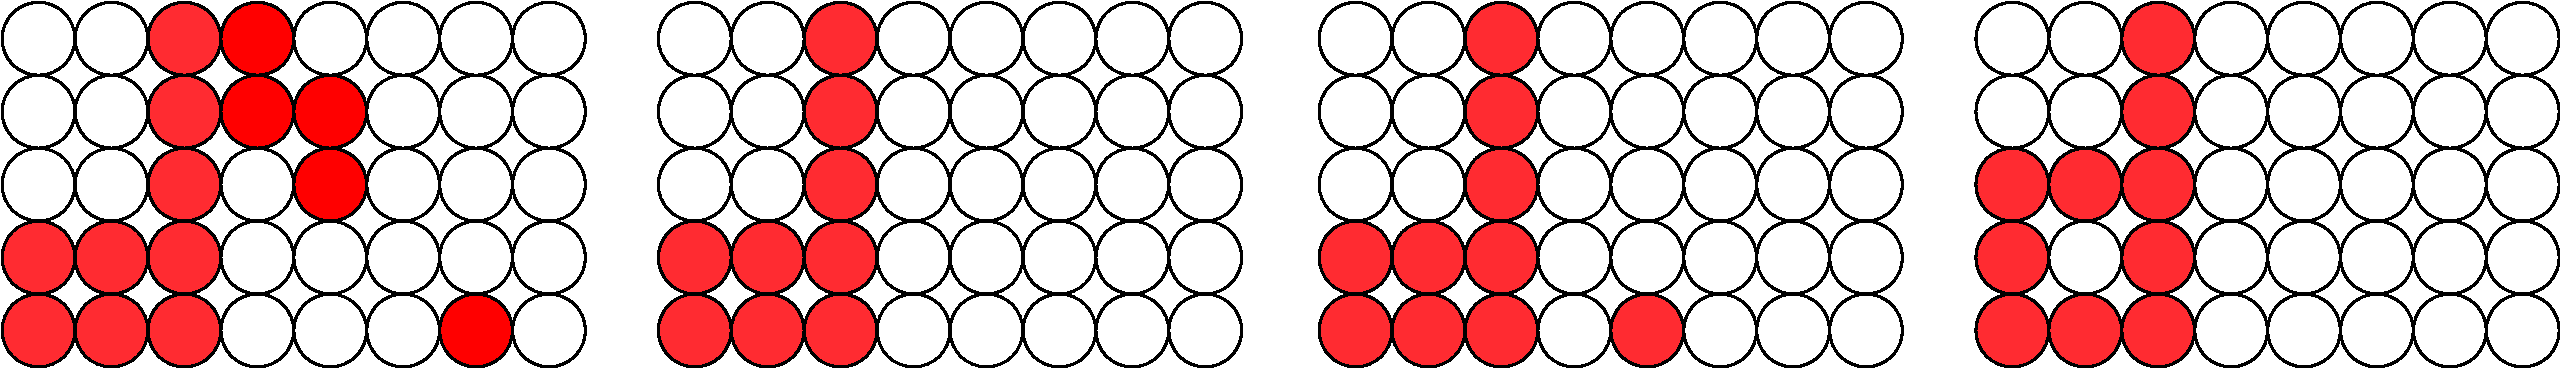
\includegraphics[width=2in]{NoteSpeed3.pdf}}\\
			Half Note Tied to Two Triplets\>\(2\ \, \myfrac{2}{3}\)\>Beats\\
			\\
			Dotted Half Note\>\(3\)\>Beats\\
			Whole Note\>\(4\)\>Beats\\
			Dotted Whole Note\>\(6\)\>Beats\>\smash{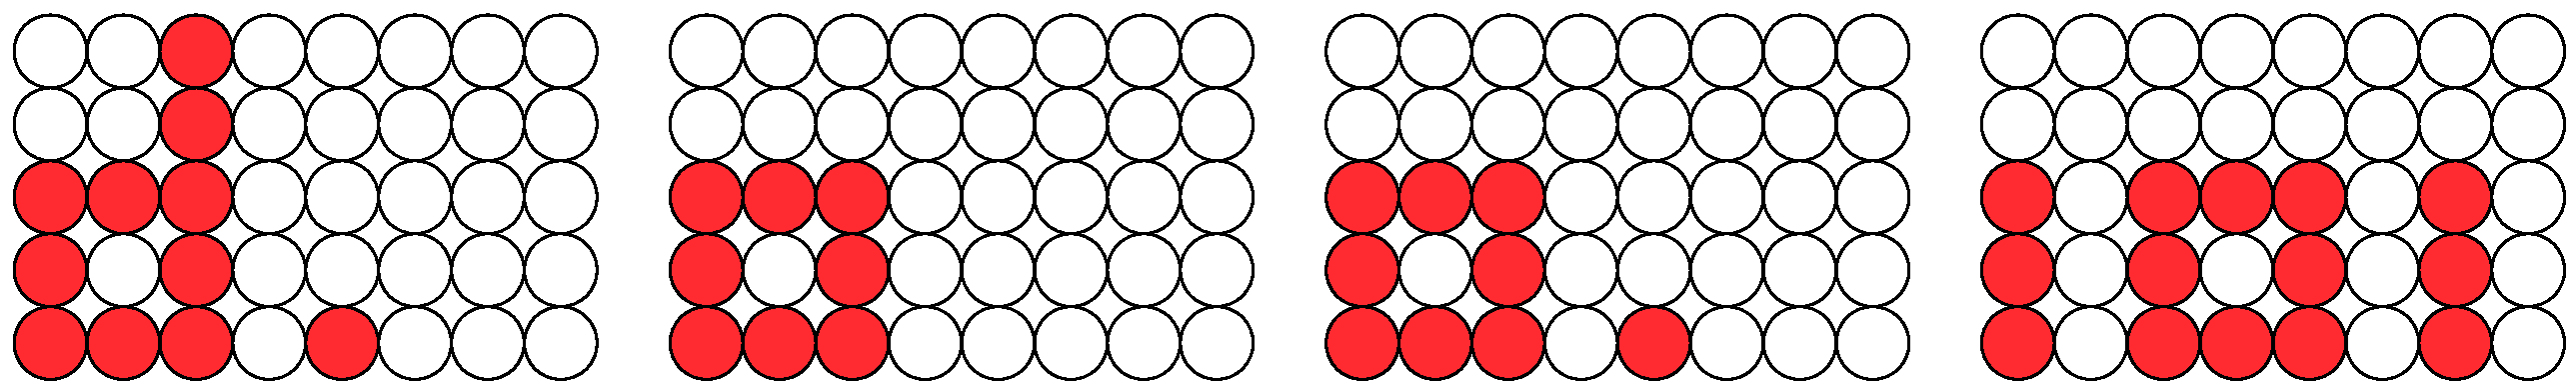
\includegraphics[width=2in]{NoteSpeed4.pdf}}\\
			Double Whole Note\>\(8\)\>Beats
			\end{tabbing}
		\end{description}
		}

	\item{\bf Swing}\\
			Swing, or {\bf syncopation}, is the degree to which every other note is delayed.  0\% means no swing at all.  100\% means so much swing that the odd note plays at the same time as the next even note.  That's a lot.
		\begin{description}
		\item{\bf \textit{Choose}}: 0\% ... 100\% (larger percentages are more swing, that is, longer delay every other note)
		\end{description}

		Swing is only applied if the Note Speed is set to thirty-second, sixteenth, eighth, quarter, or half-notes.

	\item{\bf \textit{Mega Only:}\quad Transpose}\\
		Here you can state that any notes generated by Gizmo be {\bf transposed} up or down by as much as 60 notes. If a note is transposed to the point that it exceeds the MIDI range, it is not played.  When appropriate, some applications (such as the MIDI Gauge) ignore this option. 
		\begin{description}
		\item{\bf \textit{Choose}}: \(-60\) ... 60 
		\end{description}

	\item{\bf \textit{Mega Only:}\quad Volume}\\
		Like Transpose, here you can state that any notes generated by Gizmo have their volume changed by multiplying their MIDI note velocity by some value.  If a resulting MIDI note velocity exceeds the maximum (127), it is bounded to 127.
			
			
			\begin{description}
			\item{\bf \textit{Choose}}:
			\begin{tabbing}
			1/8\\
			1/4\\
			1/2\hspace{3.65in}\smash{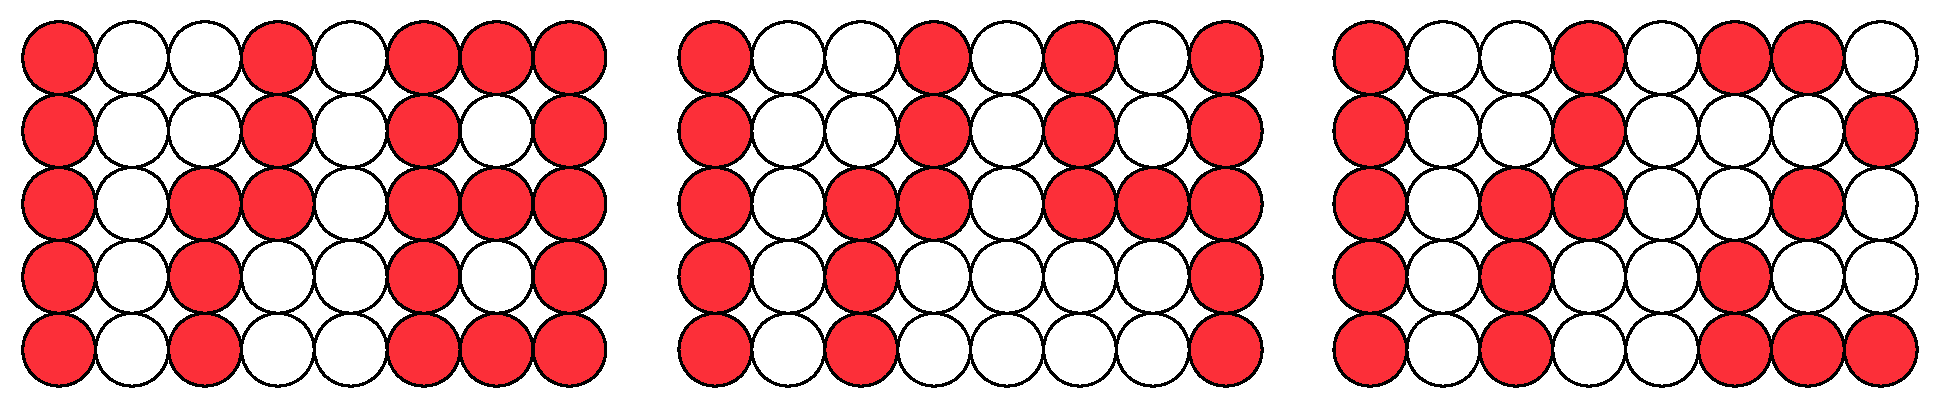
\includegraphics[width=1.7in]{fractions2.pdf}}\\
			1\qquad (default)\\
			2\\
			4\\
			8
			\end{tabbing}
		\end{description}

	\item{\bf In MIDI}\,\footnote{{\it Why aren't these called MIDI In and MIDI Out?}  Because then they'd be indistinguishable on the menu screen before the text started scrolling.}\\
		Many applications expect notes and other controls to come in via a specific input MIDI channel.  You specify it here.
		\begin{description}
		\item{\bf \textit{Choose}}: No Channel, Channels 1...16, or ALL Channels (OMNI)\hspace{0.25in}\smash{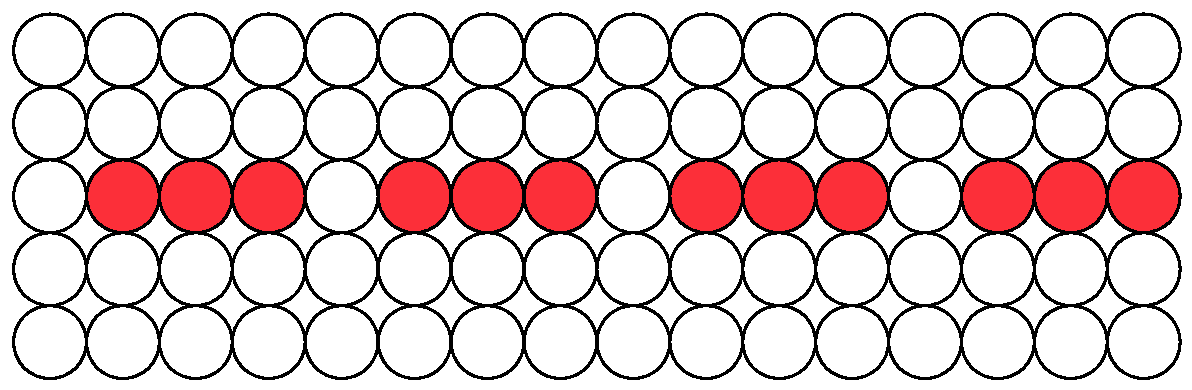
\includegraphics[width=1in]{none.pdf}}~\smash{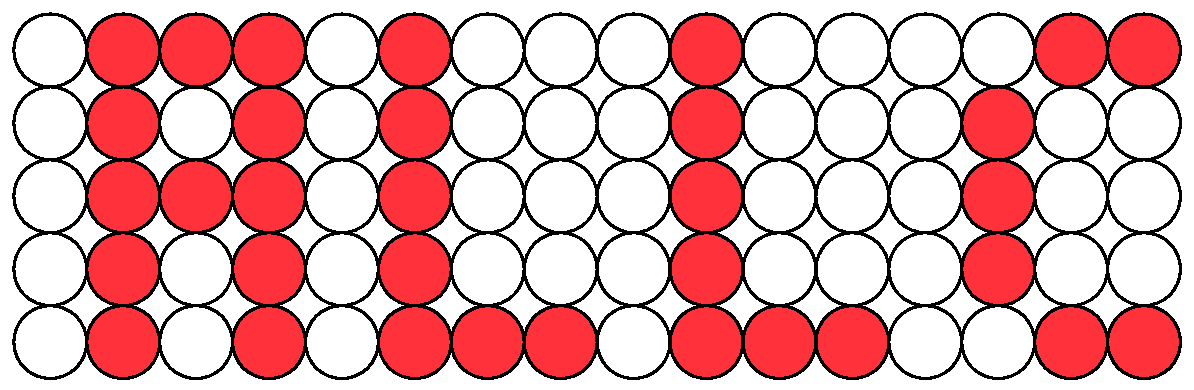
\includegraphics[width=1in]{all.pdf}}
		\end{description}
	\item{\bf Out MIDI}\\
		Many applications emit notes etc. via a specific output MIDI channel.  You specify it here.  Other applications can emit notes on several different channels, in which case this value determines the default channel used.
		\begin{description}
		\item{\bf \textit{Choose}}: No Channel, or Channels 1...16\hspace{0.5in}\smash{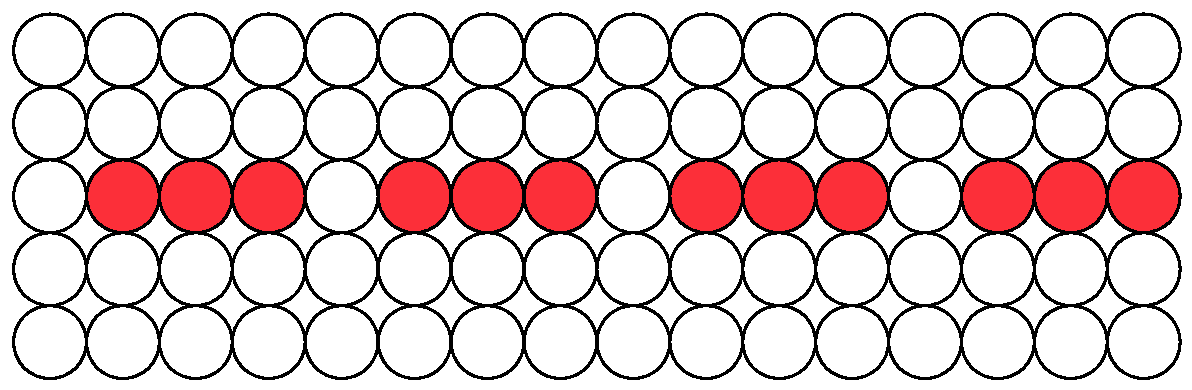
\includegraphics[width=1in]{none.pdf}}
		\end{description}
	\item{\bf Control MIDI}\\
		The arduino can be controlled via NRPN or (on the Mega) CC messages.  You specify the channel here on which it will listen for them.
		\begin{description}
		\item{\bf \textit{Choose}}: No Channel, or Channels 1...16\hspace{0.5in}\smash{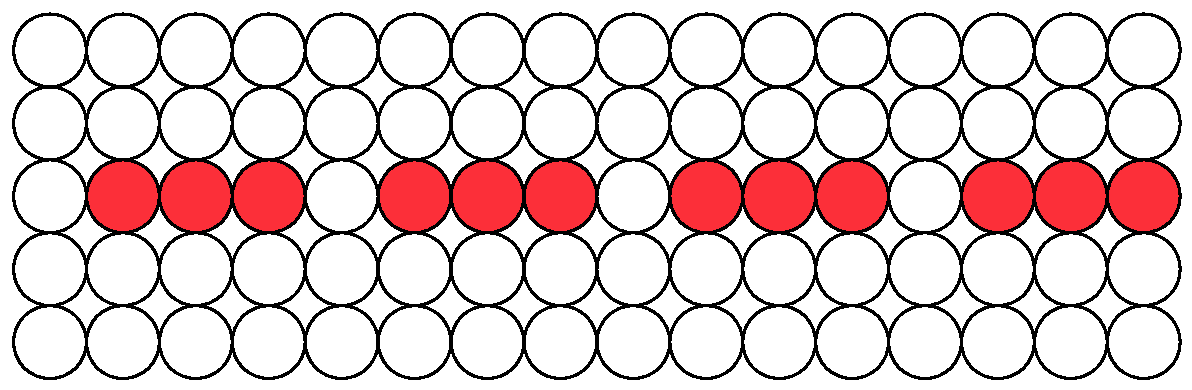
\includegraphics[width=1in]{none.pdf}}
		\end{description}
		
		The default\footnote{If you need to change these parameters, see constants (such as \texttt{CC\_LEFT\_POT\_PARAMETER}) in the file \texttt{MidiInterface.h}.  Remember, you'll want the Pot parameters to be 14-bit.} CC and NRPN Messages are (note that CC 14 and 15 are 14-bit: their LSB are sent with 46 and 47):
		
		\noindent\hspace{-1.5em}\begin{tabular}{@{}rr|lllp{2.4in}@{}}
		\multicolumn{2}{c}{\it Parameter}\\
		{\it CC}&{\it \hspace{-0.8em} NRPN}&{\it Min  Value}&{\it Max Value}&{\it MSB/LSB}&{\it Description}\\[0.1em]
		\hline\\[-0.9em]
		14&0	&0	& 1023 & MSB + LSB (46)& Turn the Left Potentiometer\\
		15&1	&0	& 1023 & MSB + LSB (47) & Turn the Right Potentiometer\\
		102&2	&0 (released)	&Not 0 (pressed) & MSB& Press/Release the Back Button\\
		103&3	&0 (released)	&Not 0  (pressed) & MSB & Press/Release the Middle Button\\
		104&4	&0 (released)	&Not 0 (pressed) & MSB & Press/Release the Select Button\\
		105&5	&Any Value	&Any Value & MSB& Toggle Bypass\\
		106&6	& Any Value &Any Value & MSB& Unlock Potentiometers.  When an NRPN message is received, normally the on-board potentiometers are locked so that turning them has no effect.  Pressing an on-board button unlocks them: so does sending this NRPN message.\\
		107&7	&	Any Value &Any Value & MSB& Start Clock.  If Gizmo's clock is stopped, resets and starts it.  When appropriate, sends a MIDI START message.\\
		108&8	& Any Value	&Any Value & MSB& Stop Clock.  If Gizmo's clock is playing, stops it.  When appropriate, sends a MIDI STOP message.\\
		109&9	&	Any Value &Any Value & MSB & Continue Clock.    If Gizmo's clock is stopped, continues it.  When appropriate, sends a MIDI CONTINUE message.\\
		\end{tabular}\\
		\\
		\\
		You can also start/stop/continue the clock via by pressing the Middle button while in the Options menu (see {\bf Starting, Stopping, and Continuing the Clock} at the end of this section).
		
	\item{\bf MIDI Clock}\\
		Gizmo can respond to a MIDI clock, ignore it, or emit its own MIDI clock.  The use of the {\bf Options\(\boldsymbol\rightarrow\)Tempo} setting will depend on the setting chosen here.

\vbox{
		\begin{description}
			\item{\bf \textit{Choose}}:
			\begin{tabbing}
			Ignore\hspace{0.5in}\=Use an internal clock but let any external MIDI clock pass through.\\
			Use\>Use an external MIDI clock and also let it pass through.\\
			Consume\>Use an external MIDI clock but don't let it pass through.\\
			Generate\>Use an internal clock and emit it as a MIDI clock.\\
			\>~~~~~~Don't let any external MIDI clock pass through.\\	
			Block\>Use an internal clock but don't emit it as a MIDI clock.\\
			\>~~~~~~Don't let any external MIDI clock pass through.\\
			\end{tabbing}
		\end{description}
}

		You can also start/stop/continue the clock via by pressing the Middle button while in the Options menu (see {\bf Starting, Stopping, and Continuing the Clock} at the end of this section), or by sending an appropriate NRPN message (see {\bf Control MIDI} earlier).

	\item{\bf Divide}\\
	If your MIDI Clock option is set to {\bf Use}, {\bf Ignore}, or {\bf Generate} (that is, something which causes Gizmo to emit MIDI Clock), then you have the option of slowing down the emitted MIDI clock by {\it dividing} it by some constant \(N\)  For example, if your clock is presently running at 120 BPM, and you're doing Generate, and \(N=3\), then Gizmo's emitted MIDI clock will be at 40BPM.   Or if you're doing Use and the incoming MIDI Clock is at 100BPM, and \(N=2\), then Gizmo will adjust this to 50BPM when sent out.  Note that Gizmo's internal applications will use the original clock speed.  Note that {\bf Bypass Mode} disables all this nonsense.
	
Why is this useful?  Here's an example scenario.  You have a sequencer on Device A which is playing a song at 120 BPM, and you want to slave another sequencer, on Device B, to it which plays its part at half that speed.  You can do this by having Device A send to Gizmo, and Gizmo send to Device B with a divided clock.

			\begin{description}
					\item{\bf \textit{Choose}}: 2 ... 16 (the value for \(N\)) when using {\bf Divide}, or None\hspace{1.45in}\smash{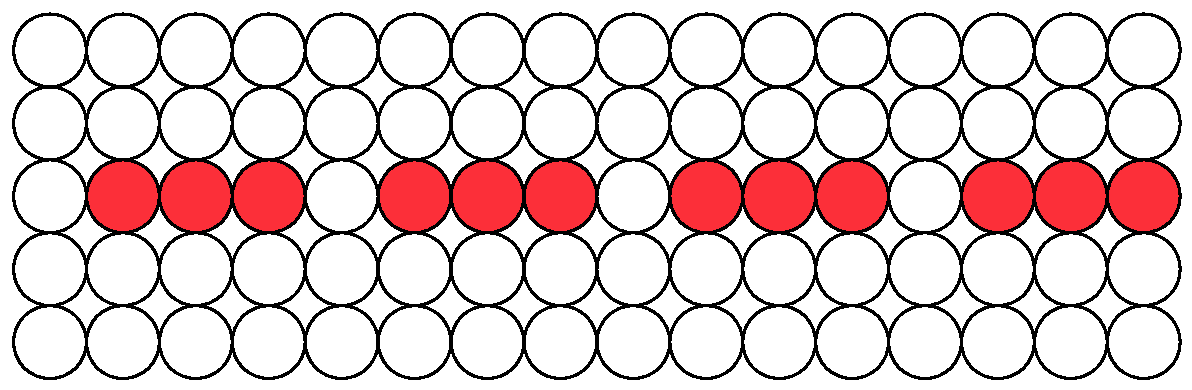
\includegraphics[width=1in]{none.pdf}}
			\end{description}


%	\begin{center}\begin{tabular}{@{}lr@{}}
%	{\it Note Speed}&{\it Divisor}\\
%					\hline\\[-0.9em]
%	
%	Eighth Triplet (Triplet 64th Note)	&1\\
%	Quarter Triplet (Triplet 32nd Note)	&2\\
%	Thirty-Second Note				&3\\
%	Half Triplet (Triplet 16th Note)		&4\\
%	Sixteenth Note					&6\\
%	Triplet						&8\\
%	Eighth Note					&12\\
%	Quarter Note					&24\\
%	Quarter Note Tied to Triplet		&32\\
%	Dotted Quarter Note				&36\\
%	Half Note						&48\\
%	Half Note Tied to Two Triplets		&64\\
%	Dotted Half Note				&72\\
%	Whole Note					&96\\
%	Dotted Whole Note				&144\\
%	Double Whole Note				&192\\
%	\end{tabular}\end{center}

		
	\item{\bf Click} or {\bf No Click}\\
		This toggles the note played by Gizmo to provide a click track for applications such as the Step Sequencer or Recorder.  If you select {\bf Click}, you will be asked to play a {\bf note}.  The note pitch and velocity form the click.  If you select {\bf No Click}, this turns off the click track.
		
\hspace{\fill}\smash{\\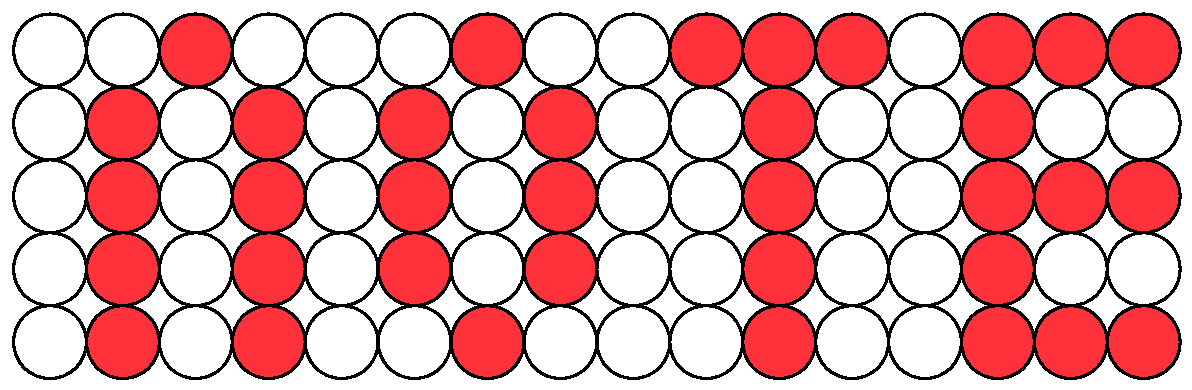
\includegraphics[width=1in]{note.pdf}}\vspace{-1.5em}

	\item{\bf Screen Brightness}\\
		This changes the brightness of the LED matrix.
		\begin{description}
		\item{\bf \textit{Choose}}: 1...16 (higher values are brighter)
		\end{description}
		
		
	\item{\bf \textit{Mega Only:}\quad Menu Delay}\\
		Gizmo often will display text (such as \texttt{SWING}) by filling the screen with the first few letters (in this case, \texttt{SWI}), then {\it delaying} for a certain interval, then scrolling through the whole word horizontally. You can specify how long that delay is.
		
		\clearpage
		
		\begin{description}
			\item{\bf \textit{Choose}}:
			\begin{tabbing}
			0\hspace{2em}\=Seconds\hspace{1in}\=(scroll immediately)\\
			1/8\>Seconds\\
			1/4\>Seconds\\
			1/3\>Seconds\>\hspace{1.5in}\=\smash{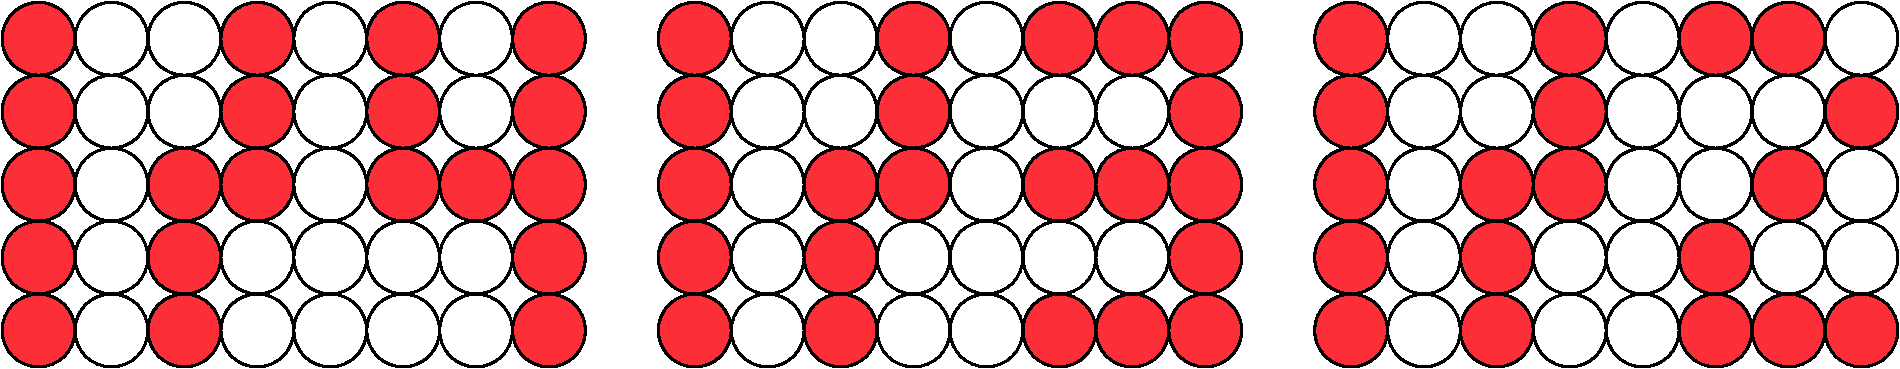
\includegraphics[width=2in]{fractions.pdf}}\\
			1/2\>Seconds\\
			1\>Second\>(default)\\
			2\>Seconds\\
			3\>Seconds\\
			4\>Seconds\\
			8\>Seconds\\
			\(\infty\)\>Seconds\>(never scroll)\>\smash{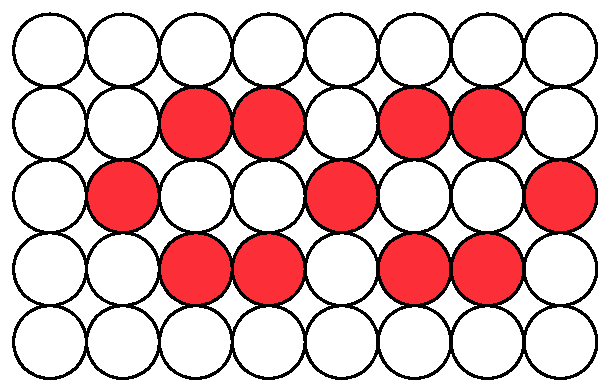
\includegraphics[width=0.48in]{infinity}}
			\end{tabbing}
		\end{description}


	\item{\bf  \textit{Mega Only:}\quad CV+Velocity \textit{or} CV+Aftertouch \textit{or} No CV}\\
		Toggles whether Gizmo will send control voltage and gate information.  If {\bf CV+Velocity}, then control voltage will be sent out DAC A (I2C address 0x62), velocity will be sent out DAC B (I2C address 0x63), and digital pin 8 will be set HIGH (5V) when a note is played (or LOW (0V) when a note is released), thus acting as a Gate.\footnote{As mentioned in an earlier footnote, Gizmo assumes you're DACs of this kind: https:/\!/www.adafruit.com/product/935} If {\bf CV+Aftertouch}, then the same is done except that aftertouch will be sent out DAC B instead of velocity.  If {\bf No CV}, then nothing is sent.  Pitch Bend at present has no effect.	\footnote{Note that at present if you have set either knob in the Controller to control voltage, that DAC will be unavailable even outside the Controller.  I'll fix that soon.}
		
	\item{\bf The About Screen}\\
		Presently says:\quad \texttt{GIZMO V2 (C) 2017 BY SEAN LUKE}
	\end{description}

	\section{Starting, Stopping, and Continuing the Clock (on the Mega)}
	\label{startingclock}

		You can start, stop, and continue the clock via NRPN/CC as discussed earlier (see {\bf Control MIDI} in Section \ref{options}).   But there's another ``secret'' way to do it on the Mega, using Gizmo's buttons.  If you are in the Options menu, long-press the Middle Button: this toggles {\bf starting} or {\bf stopping} the clock.  And if you long-press the Select button, you can toggle {\bf continuing} or {\bf stopping} the clock.  Remember that you can also get to the Options menu from inside the Arpeggiator, Step Sequencer, or Recorder.
		
		Neither long-pressing the Middle Button, nor using NRPN to start/stop/continue, will do anything if the MIDI Clock is set to {\bf Use, Divide,} or {\bf Consume} (in which case the MIDI Clock is out of your control).  See {\bf MIDI Clock} in Section \ref{options}.
				
		Note that starting and stopping the clock doesn't mean that an application starts or stops playing.  However, the Start message {\it will} cause applications to reset themselves to the beginning when appropriate.   This means that if you want to start/stop/pause/continue the Step Sequencer (for example), you can do it as follows: first stop the clock, then start the sequencer playing.  Note that it won't play because there's no clock pulses.  But now you can start, stop, and pause/continue the sequencer by controlling the Start/Stop/Continue clock messages directly.
		
		Manually stopping and starting the clock can produce results which look like bugs, but aren't, so you have think about the effects.  For example, if you're in {\bf Generate Clock} mode and you've manually stopped the clock, and you go into the Step Sequencer and start playing, nothing will happen. More than once this has confused me enough to look through the code thinking I'd written an error.
		
	\section{The Internal Clock}
	\label{internalclock}

The Arduino has an internal clock with 32 bits, yielding a maximum of 42,949,672,95 ticks (one tick per microsecond) before it rolls back over to 0.  This sounds like a lot, but it's not: it's a bit over an hour.\footnote{71.5827882666 minutes to be exact.}  This means that once an hour, Gizmo might do something odd, if you're using the internal clock.  Most likely it could drop a single pulse (1/24 of a quarter note), so it might be off by that much with respect to other instruments synced to it.  You've been warned.


\section{Development Status}

\begin{center}
{
\setlength\extrarowheight{0.3em}
\begin{tabular}{@{}llllp{2.8in}@{}}
&&\multicolumn{2}{c}{\it Testing}&\\[0.1em]
\cline{3-4}\\[-0.9em]
{\it Item} & {\it Coded} & {\it Cursory} & {\it Significant} & {\it Known Bugs and Issues}\\[0.1em]
		\hline\\[-1.5em]
Arpeggiator& $\checkmark$ & $\checkmark$ & $\checkmark$  & \\
Step Sequencer& $\checkmark$ & $\checkmark$ & $\checkmark$ & Occasionally the beat doesn't match up with the play cursor; this particularly happens under Swing.  I've not been able to track it down.\\
Recorder& $\checkmark$ & $\checkmark$ & $\checkmark$ & Rarely a note will get stuck after recording: appears that a NOTE OFF message isn't getting matched with the ID of the corresponding NOTE ON message when entered into memory.  
I also think there may be a bug causing chords near the start of the song to be rushed a bit.  Perhaps timing is being delayed for some reason?\\
Gauge& $\checkmark$ & $\checkmark$ &\\ 
Controller& $\checkmark$ & $\checkmark$ & & Voltage and Aftertouch untested.  Pitch Bend displays correctly but MIDI output is untested.\\ 
NRPN Control  &  $\checkmark$ & $\checkmark$ &  $\checkmark$ &\\
Transposition / Volume  &  $\checkmark$ & $\checkmark$ &  $\checkmark$ &\\
Brightness / Delay  &  $\checkmark$ & $\checkmark$ &  $\checkmark$ &\\
Tempo / Note Speed &  $\checkmark$ & $\checkmark$ &  $\checkmark$ &\\
MIDI In/Out Channels &  $\checkmark$ & $\checkmark$ &  & No test of OMNI yet\\
Bypass &  $\checkmark$ & $\checkmark$ &  $\checkmark$ &\\
Display Subsystem  &  $\checkmark$ & $\checkmark$ &  $\checkmark$ &\\
Timing  Subsystem &  $\checkmark$ & $\checkmark$ &  $\checkmark$ &\\
Interface Utilities &  $\checkmark$ & $\checkmark$ &  $\checkmark$ & \\
Storage Facility &  $\checkmark$ & $\checkmark$ &  $\checkmark$ &\\
MIDI Clock Control& $\checkmark$ & $\checkmark$ & &Odd things may happen when changing the clock control option while an external clock is active.\\
Clock Division&$\checkmark$&$\checkmark$& &\\
Keyboard Splitting& $\checkmark$ & $\checkmark$  & & Works well but the fade option is perhaps a bit unnecessary and weird.\\
Thru Facility & $\checkmark$ & $\checkmark$ & & \\
Control Voltage& $\checkmark$ & & & Untested\\
Tap Tempo & $\checkmark$ & $\checkmark$& & Seems to work, but might be better to average in tempos.  This would require floating point probably, which would be too big for the Uno.\\
Measure Counter & $\checkmark$ & $\checkmark$& & Seems to work.  MIDI clock response has not been tested.
\end{tabular}
}
\end{center}


\end{document}
